\apendice{Especificación de Requisitos}
\label{s:anexo-B}

\section{Introducción}

La fase de análisis es una etapa fundamental en el ciclo de vida del desarrollo ya que permite entender los requerimientos del cliente e identificar los componentes necesarios para entregar un producto adecuado.

Durante esta fase, el equipo de desarrollo se reune con el cliente (o con su representante el \textit{product owner}) y, tras realizar diversas entrevistas, se recoge lo que este espera de la aplicación. Además, el equipo de desarrollo analizará todos los requisitos no relacionados con la funcionalidad (como puede ser seguridad, escalabilidad, rendimiento, etc.) que se puedan deducir de dichas conversaciones.

Debido a la importancia que tiene esta fase, se ha experimentado una evolución con los años y se han propuesto distintas aproximaciones en función de las metodologías utilizadas. Entre ellas:

\begin{itemize}
	\item \textbf{Metodologías tradicionales}: estas metodologías realizan la captura de los requerimientos en fases tempranas del desarrollo, realizando una <<fotografía>> exacta (e, idealmente, inmutable) de lo que el usuario necesita. Para ello, se hace uso de requisitos funcionales y no funcionales que se documentan en un formato estructurado y definido en estándares. Un ejemplo de especificación es el estándar \texttt{IEEE 830}~\cite{ieee830}, donde se implora que los requisitos han de ser claros, precisos, medibles, coherentes, completos, factibles, específicos y verificables.
	
	\item  \textbf{Metodologías ágiles}: en contraposición, las metodologías ágiles tratan de ser flexibles y adaptarse al usuario (ya que, muchas veces, es común que no tenga claro en etapas tempranas de desarrollo lo que realmente necesita). Para ello utilizan las denominadas historias de usuario, que son breves descripciones de las funcionalidades que el usuario necesita para realizar una tarea específica. Estos documentos se recogen en estructuras tabulares y se almacenan en el \textit{product backlog}, que lejos de ser una <<fotografía>>, es una lista <<viva>> que se actualiza y prioriza en función de las necesidades del cliente. 
\end{itemize}


Aunque en un proyecto real puede no resultar óptimo realizar una <<mezcla>> de metodologías, debido a las peculiares características de este (equipo de un desarrollador) y a que se solicita la inclusión de requisitos funcionales y no funcionales de una manera más tradicional en la memoria, se ha hecho uso de ambos métodos de documentación (complementados, además, mediante prototipos expuestos en la sección~\ref{s:mockups}). Por lo tanto, se realizará una especificación de requisitos clásica (expuesta en la sección~\ref{s:cat-requisitos} y desarrollada en la sección~\ref{s:requisitos}) complementada, a modo ilustrativo, con alguna historia de usuario extraída de las entrevistas con el \textit{product owner} (sección~\ref{s:hu}). 

Cabe destacar que durante el desarrollo real se ha utilizado una metodología ágil mediante el uso de \textit{sprints} como se ha expuesto en la sección~\ref{s:planificacion-sprints}.

\section{Objetivos generales}

En este proyecto se han definido distintos objetivos que pueden ser resumidos en los siguientes puntos:
\begin{enumerate}
	\item Implementación y validación de algoritmos de aprendizaje semisupervisado: en concreto el \textit{co-forest}, el \textit{democratic-co learning} y el \textit{tri-training}.
	\item Aplicación del \textit{machine learning} a la solución de un problema real relacionado con la ciberseguridad: se ha escogido la detección de \textit{phishing} y detección de ataques en sistemas de recomendación, aunque esta última ha sido descartada por su bajo desempeño.
	\item Desarrollo de una herramienta que permita poner al servicio de la comunidad el conocimiento desarrollado: se ha decidido desarrollar un analizador de \textit{phishing} en formato página \textit{web}, permitiendo además administración avanzada de modelos de \textit{machine learning} e instancias de aprendizaje (URLs legítimos y fraudulentos).
\end{enumerate}

Como se puede intuir, los dos primeros están enfocados a la investigación mientras que el último es una tarea de desarrollo. Por este motivo, este anexo se centrará principalmente en el tercer punto.

\section{Usuarios}
\label{s:usuarios}

En las metodologías ágiles no sólo es necesario definir las funcionalidades, sino también quién las realiza. Por ello, se introducen a continuación los distintos usuarios de la página \textit{web} desarrollada, aunque sus funciones completas se pueden observar en el diagrama de casos de uso~\ref{b:diagrama-cu}.

\begin{itemize}
	\item \textbf{Visitante}: se trata de un navegante que accede a la \textit{web}. En este caso, las funcionalidades que tiene disponibles son más limitadas, ya que únicamente se le permite analizar URLs y visualizar los resultados.
	\item \textbf{Usuario registrado}: un usuario registrado (rol <<estándar>>) tiene acceso a funcionalidades colaborativas. Es decir, además de poder escanear URLS, tiene permiso para reportar enlaces que sepa que son legítimos o \textit{phishing}. Estos serán revisados por administradores y etiquetados (de forma que pertenezcan a una lista blanca o a una lista negra). Además, también podrán notificar análisis incorrectos. De esta forma, si un usuario piensa que una URL es, por ejemplo, \textit{phishing}, y los modelos predicen que se trata de un enlace legítimo, puede notificarlo. Este aviso llegará a los administradores, quienes podrán examinar la instancia e incluirla en el \textit{dataset} para ser estudiada por modelos futuros y mejorar el rendimiento de la aplicación.
	\item \textbf{Administrador}: los usuarios que tengan este rol tendrán acceso a la funcionalidad completa de la \textit{web}. Podrán crear nuevos modelos de aprendizaje y entrenarlos con las instancias que consideren, además de editar los existentes. También podrán revisar todas las notificaciones y reportes de usuarios de la aplicación e incluir nuevas instancias en el \textit{dataset}, además de modificar las existentes.
\end{itemize}

\section{Catálogo de historias de usuario}
\label{s:hu}

\begin{table}
	\scalebox{0.80}{
	\begin{tabular}{@{}p{3em} p{4em} p{5em} p{9em} p{14em}@{}}		
	\toprule
	\textbf{ID} & \textbf{Como} & \textbf{Quiero} & \textbf{Para} & \textbf{Aceptación}\\
	\midrule
		HU-1 & Visitante & Analizar URLs & Saber si un enlace es fraudulento (\textit{phishing}) o legítimo & La página debe mostrar el resultado tras el análisis haciendo uso de técnicas visuales como gráficos interactivos.
		
		La \textit{web} debe informar si no es posible mediante un mensaje ilustrativo.\\\\
		HU-2 & Visitante & Poder registrarme & Crear una cuenta en la aplicación & La cuenta es persistente y se puede acceder a ella. \\\\
		HU-3 & Usuario registrado & Poder iniciar sesión & Acceder a más funcionalidades & Al introducir credenciales correctas se accede a una cuenta y se desbloquean opciones colaborativas. \\\\
		HU-4 & Usuario registrado & Reportar URLs & Que sean incluídas en una lista blanca o negra & Existe un lugar donde reportar URLs cuando se está seguro de la clase a la que pertenecen.\\\\
		HU-5 & Usuario registrado & Notificar análisis incorrectos & Que las instancias sean revisadas y poder mejorar los algoritmos de ML & Existe un botón con el que se reporta automáticamente que se considera que un análisis ha fallado.\\\\
		HU-6 & Adminis- trador & Administrar instancias (URLs) & Poder mantener un dataset actualizado & Se pueden añadir instancias.
		
		Se pueden generar ficheros \texttt{csv} con las instancias disponibles.
		
		Se pueden modificar instancias.
		
		Se pueden consultar las instancias reportadas por los usuarios.\\\\
		HU-7 & Adminis- trador & Administrar modelos de \textit{machine learning} & Que estén disponibles en la página y puedan ser utilizados por los usuarios para realizar análisis & Se pueden crear nuevos modelos desde la web.
		
			Se pueden probar modelos existentes.
			
			Se pueden eliminar modelos existentes.
		\\
	\bottomrule
	\end{tabular}
	}
	\caption[Historias de usuario: entrevista con el \textit{product owner}]{Historias de usuario recogidas durante las entrevistas con el \textit{product owner}}
	\label{hu:estructura-tabular}
\end{table}

A modo ilustrativo y con el fin de realizar una memoria lo más completa posible (coherente con las metodologías ágiles), se facilitan en la tabla~\ref{hu:estructura-tabular} algunas historias de usuario tomadas durante las entrevistas con el \textit{product owner}. Sin embargo, el catálogo completo de requisitos se encuentra en el apartado~\ref{s:cat-requisitos}.

\section{Prototipado}
\label{s:mockups}

Como es conocido, en el mundo del desarrollo \textit{software} suele haber una diferencia en el entendimiento de una aplicación por parte del cliente y del equipo de desarrollo que puede desembocar en malentendidos que causen retrasos temporales y pérdidas económicas.

Con el fin de reducir dichas desventajas y realizar un diseño que se adapte a los requerimientos del usuario, se ha decidido realizar una fase de prototipado durante las entrevistas del producto. Esto ha permitido identificar posibles diferencias entre el equipo del desarrollo y el cliente (representado por el \textit{product owner}), facilitando la comunicación y colaboración entre ambas partes.

Se adjuntan a continuación los diferentes prototipos de la \textit{web} para el analizador de \textit{phishing} realizados durante esta fase.


\begin{figure}[h]
	\caption{Prototipo: página principal}
	\centering
	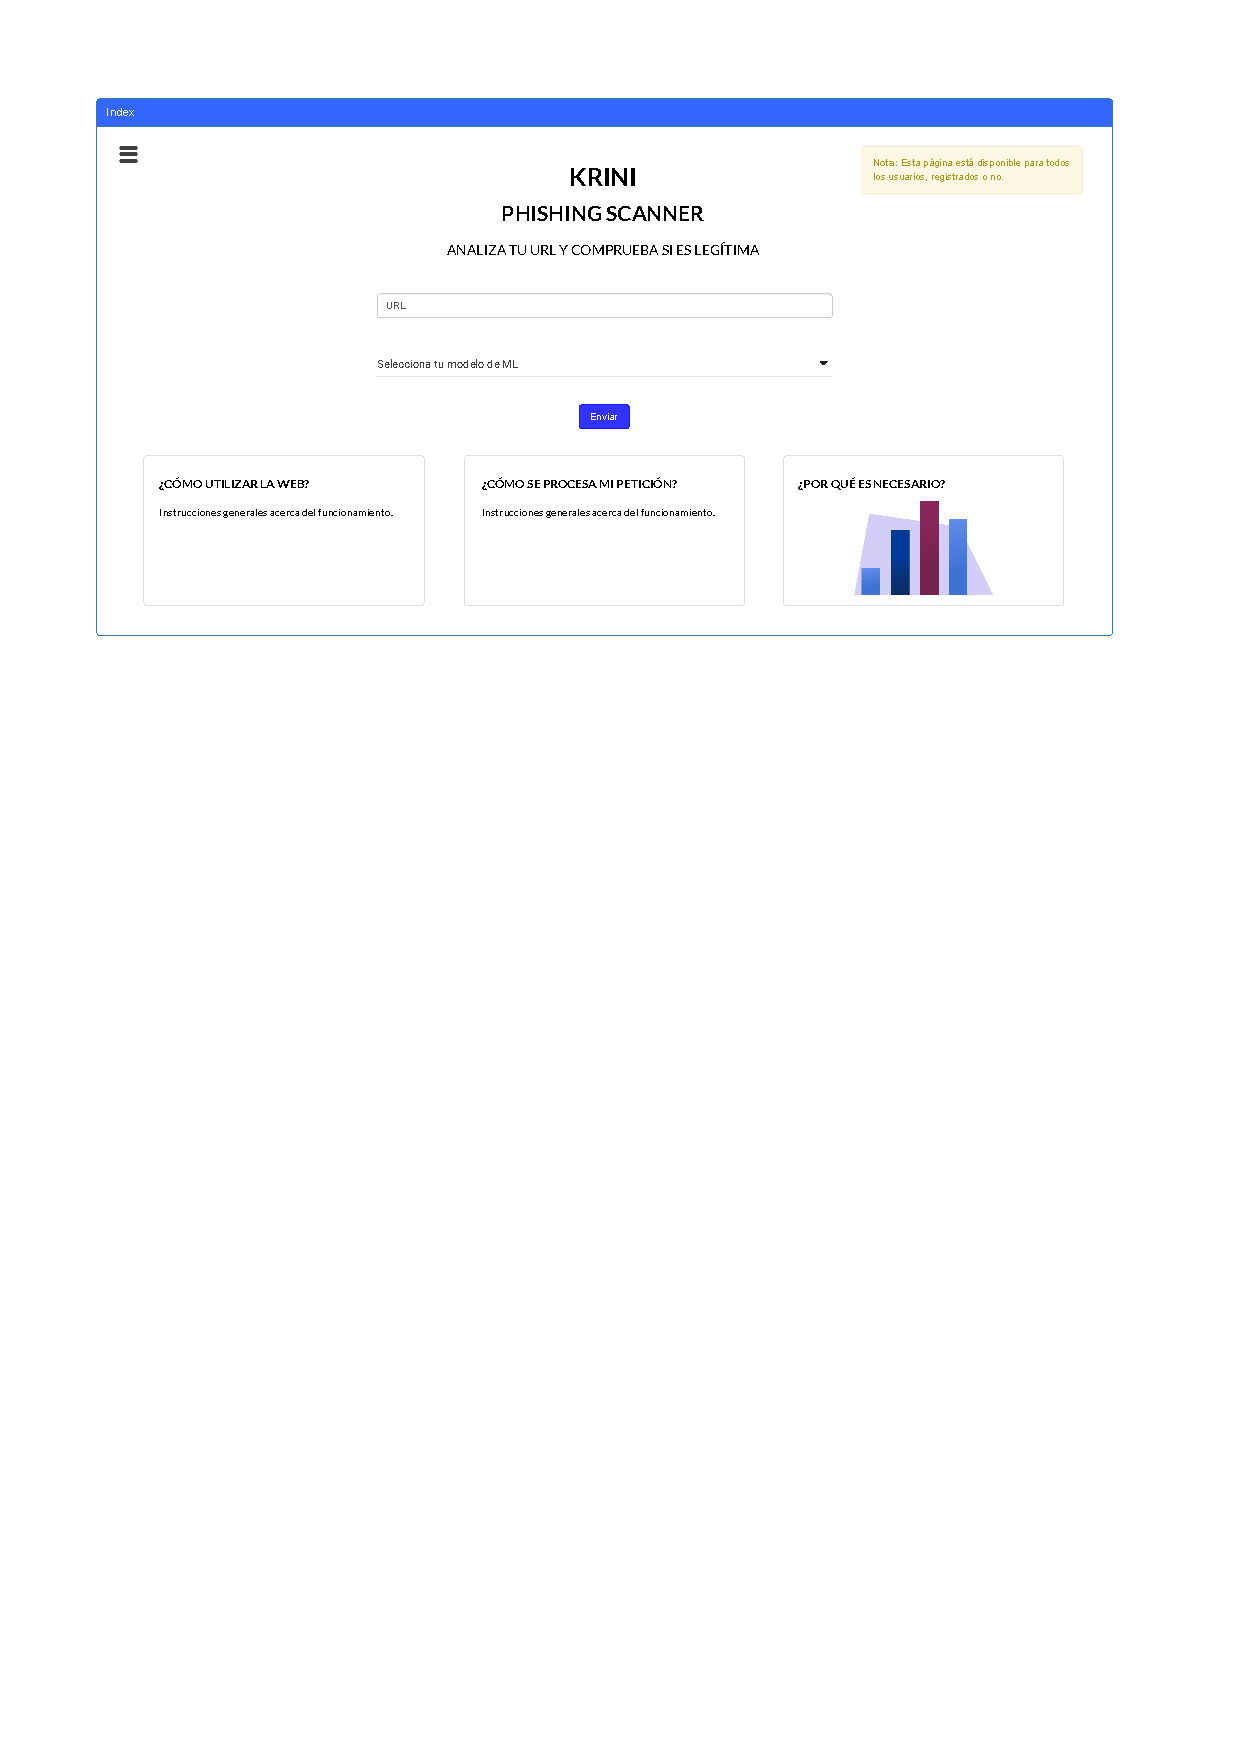
\includegraphics[width=\textwidth]{../img/anexos/mockups/1-mockups-index}
	\label{mock:index}
\end{figure}

\begin{figure}[h]
	\caption{Prototipo: \textit{dashboard}}
	\centering
	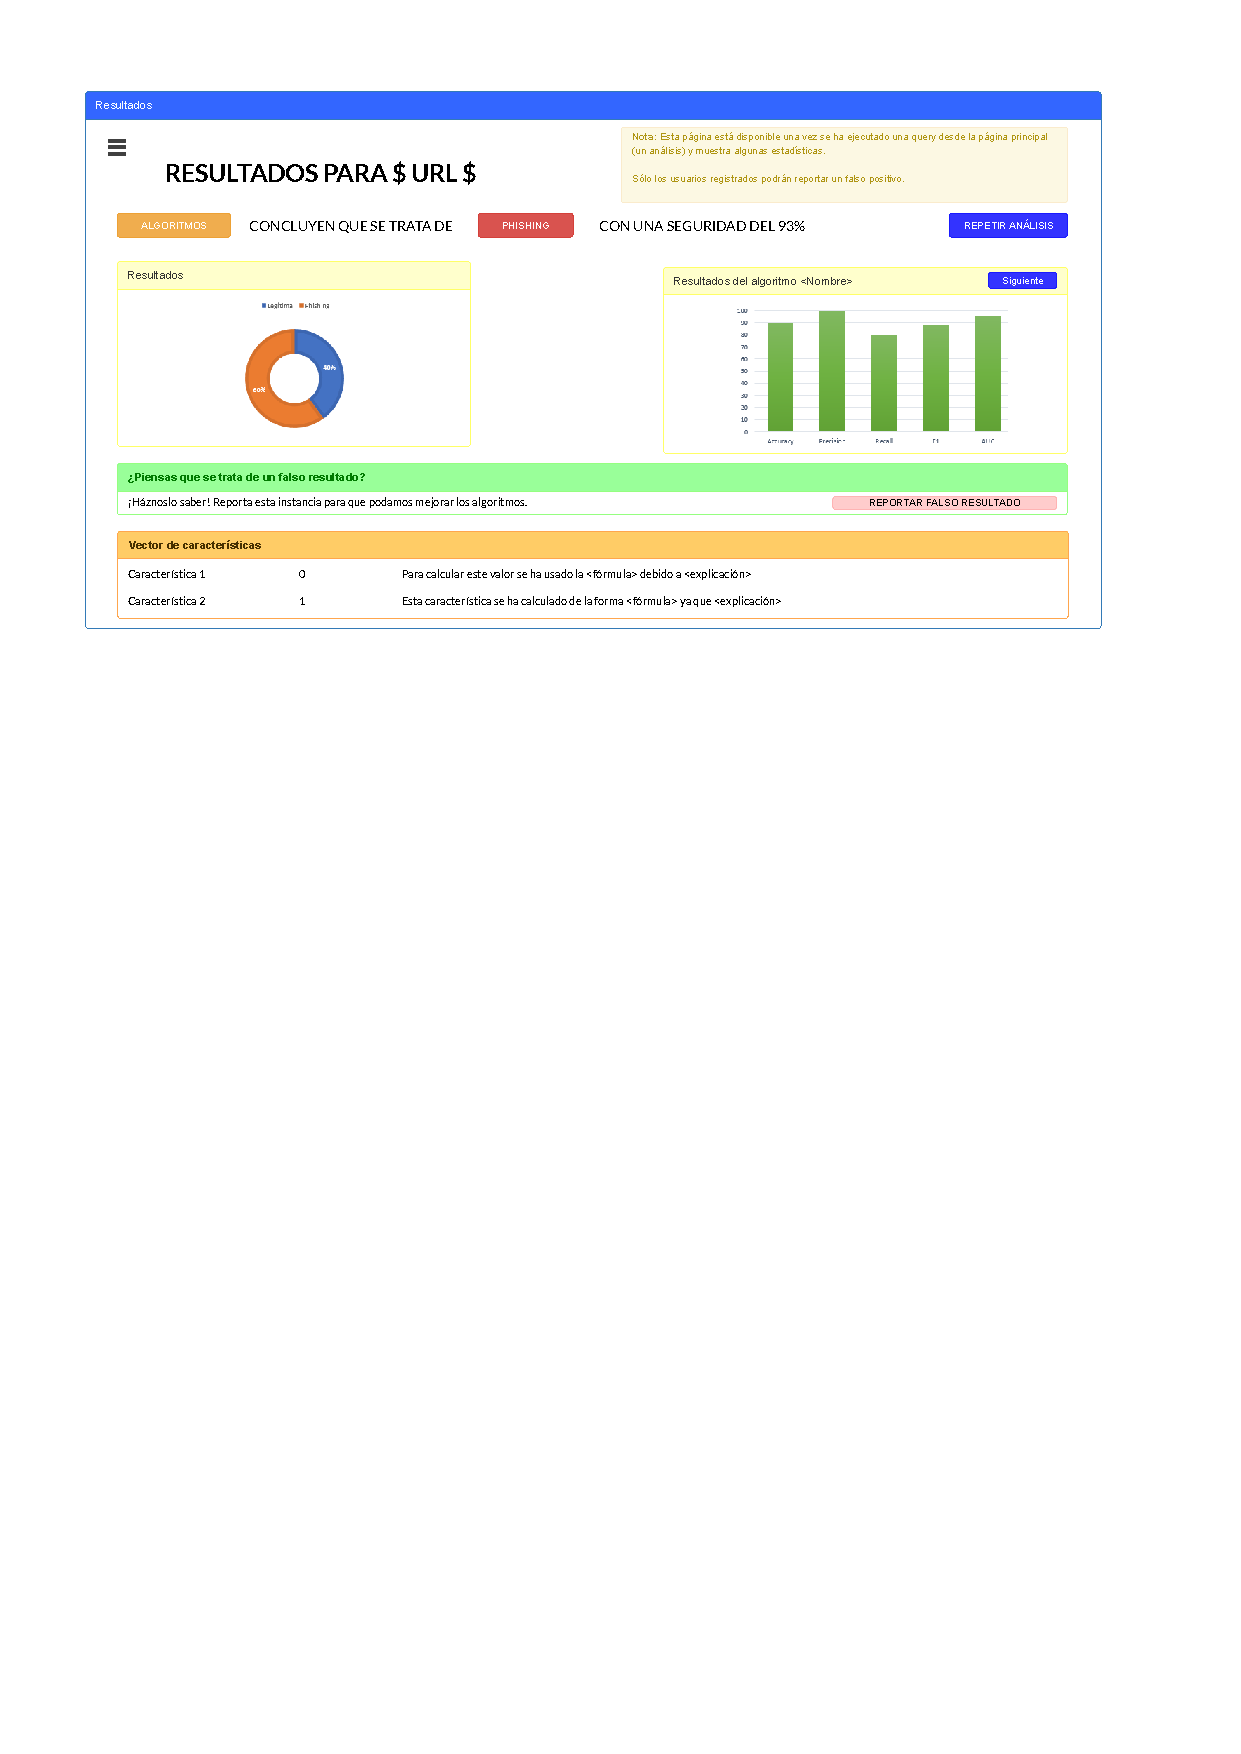
\includegraphics[width=\textwidth]{../img/anexos/mockups/2-mockups-dashboard}
	\label{mock:dashboard}
\end{figure}

\begin{figure}[h]
	\caption{Prototipo: perfil del usuario}
	\centering
	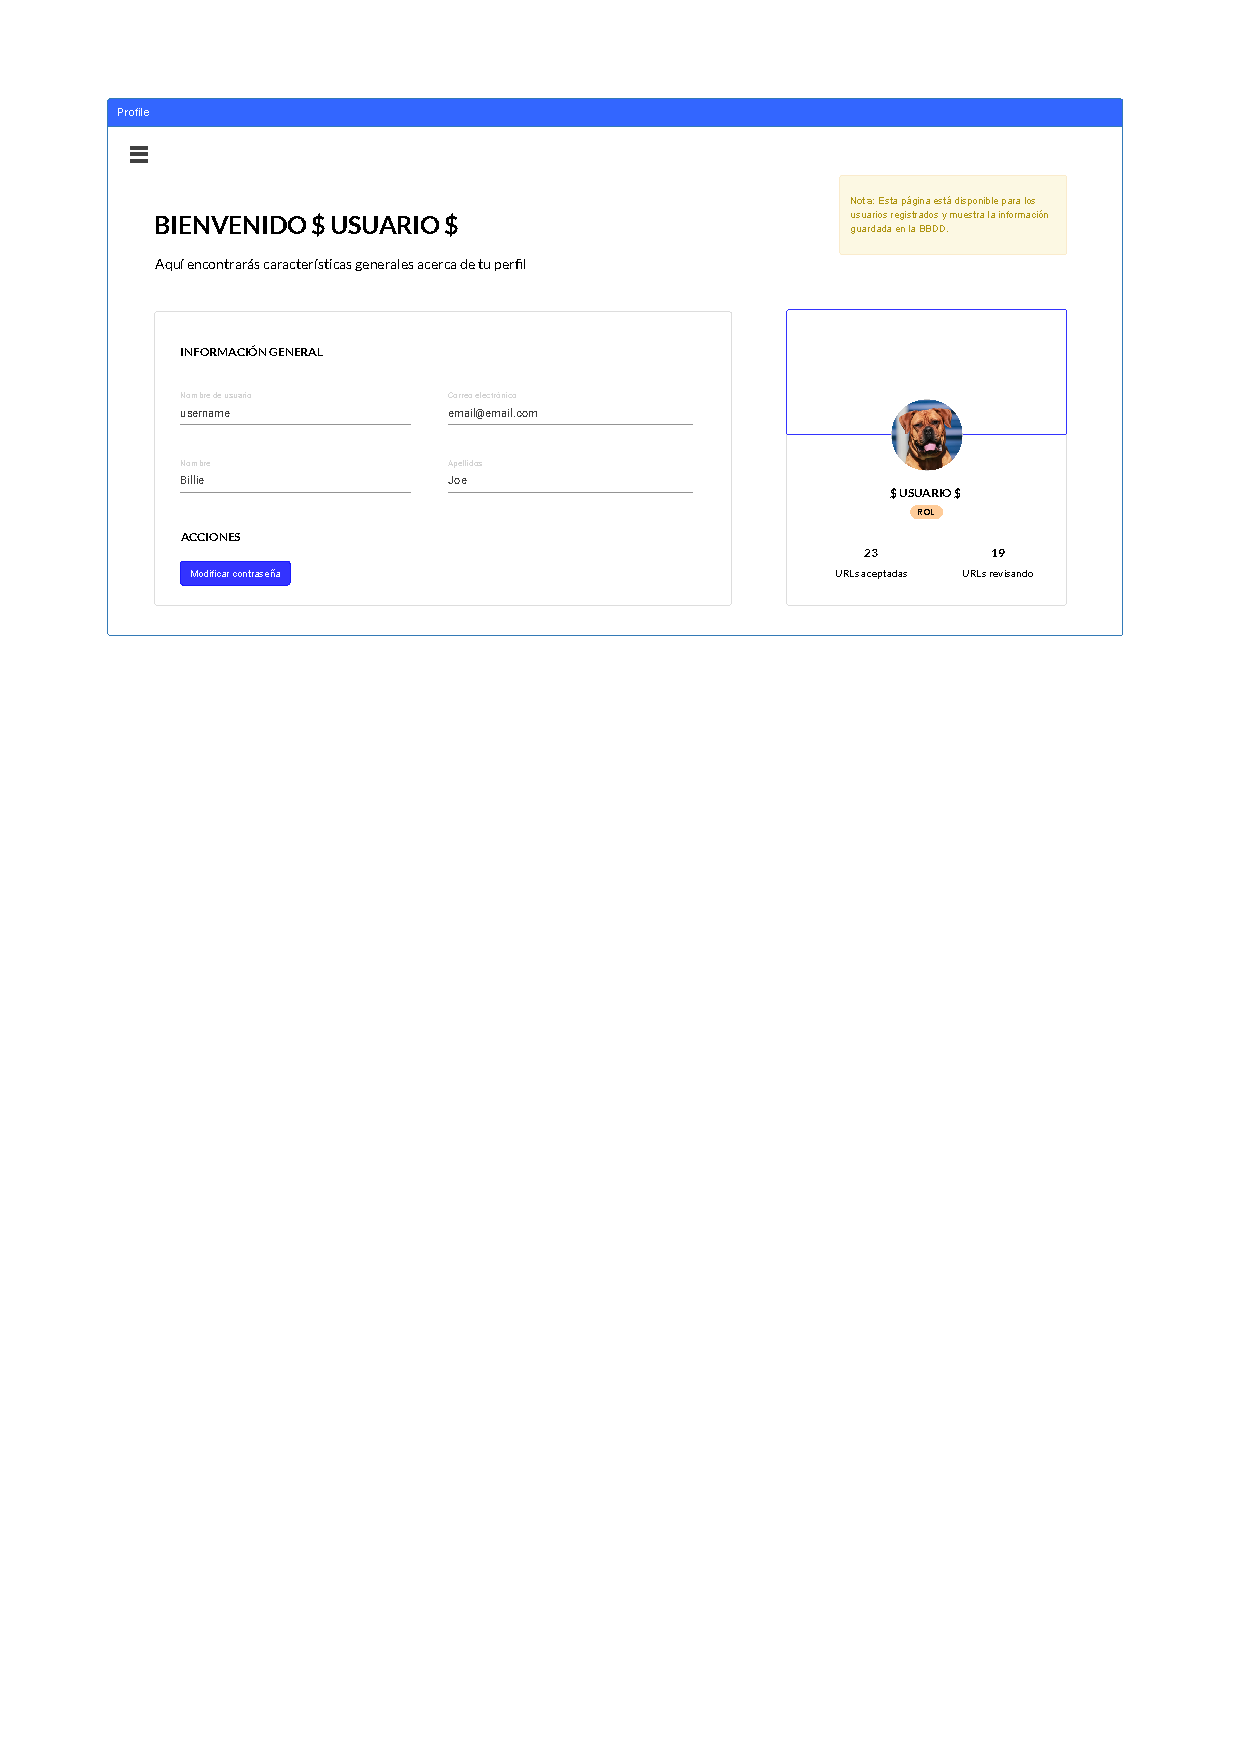
\includegraphics[width=\textwidth]{../img/anexos/mockups/4-mockups-profile}
	\label{mock:profile}
\end{figure}

\begin{figure}[h]
	\caption{Prototipo: reportar una URL}
	\centering
	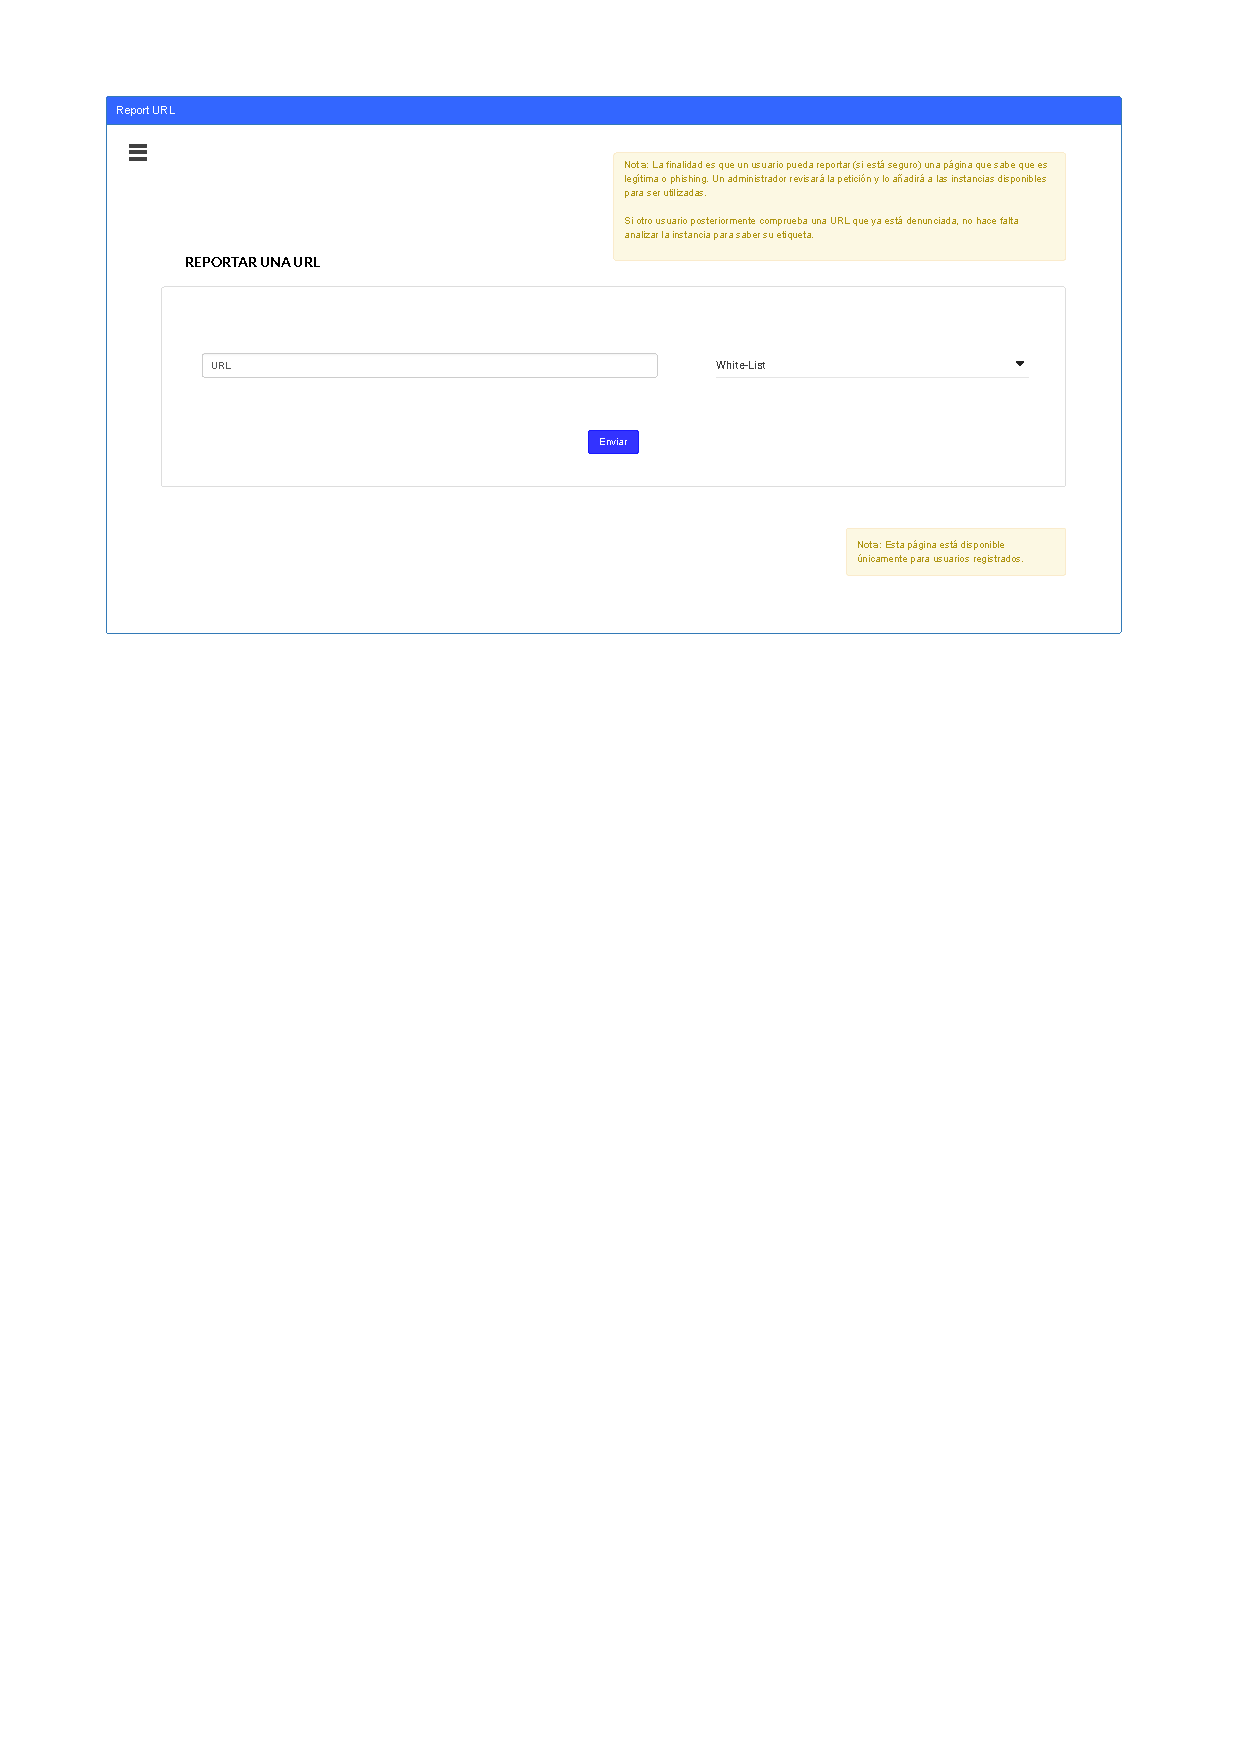
\includegraphics[width=\textwidth]{../img/anexos/mockups/3-mockups-report_url}
	\label{mock:report_url}
\end{figure}

\begin{figure}[h]
	\caption{Prototipo: administración de modelos}
	\centering
	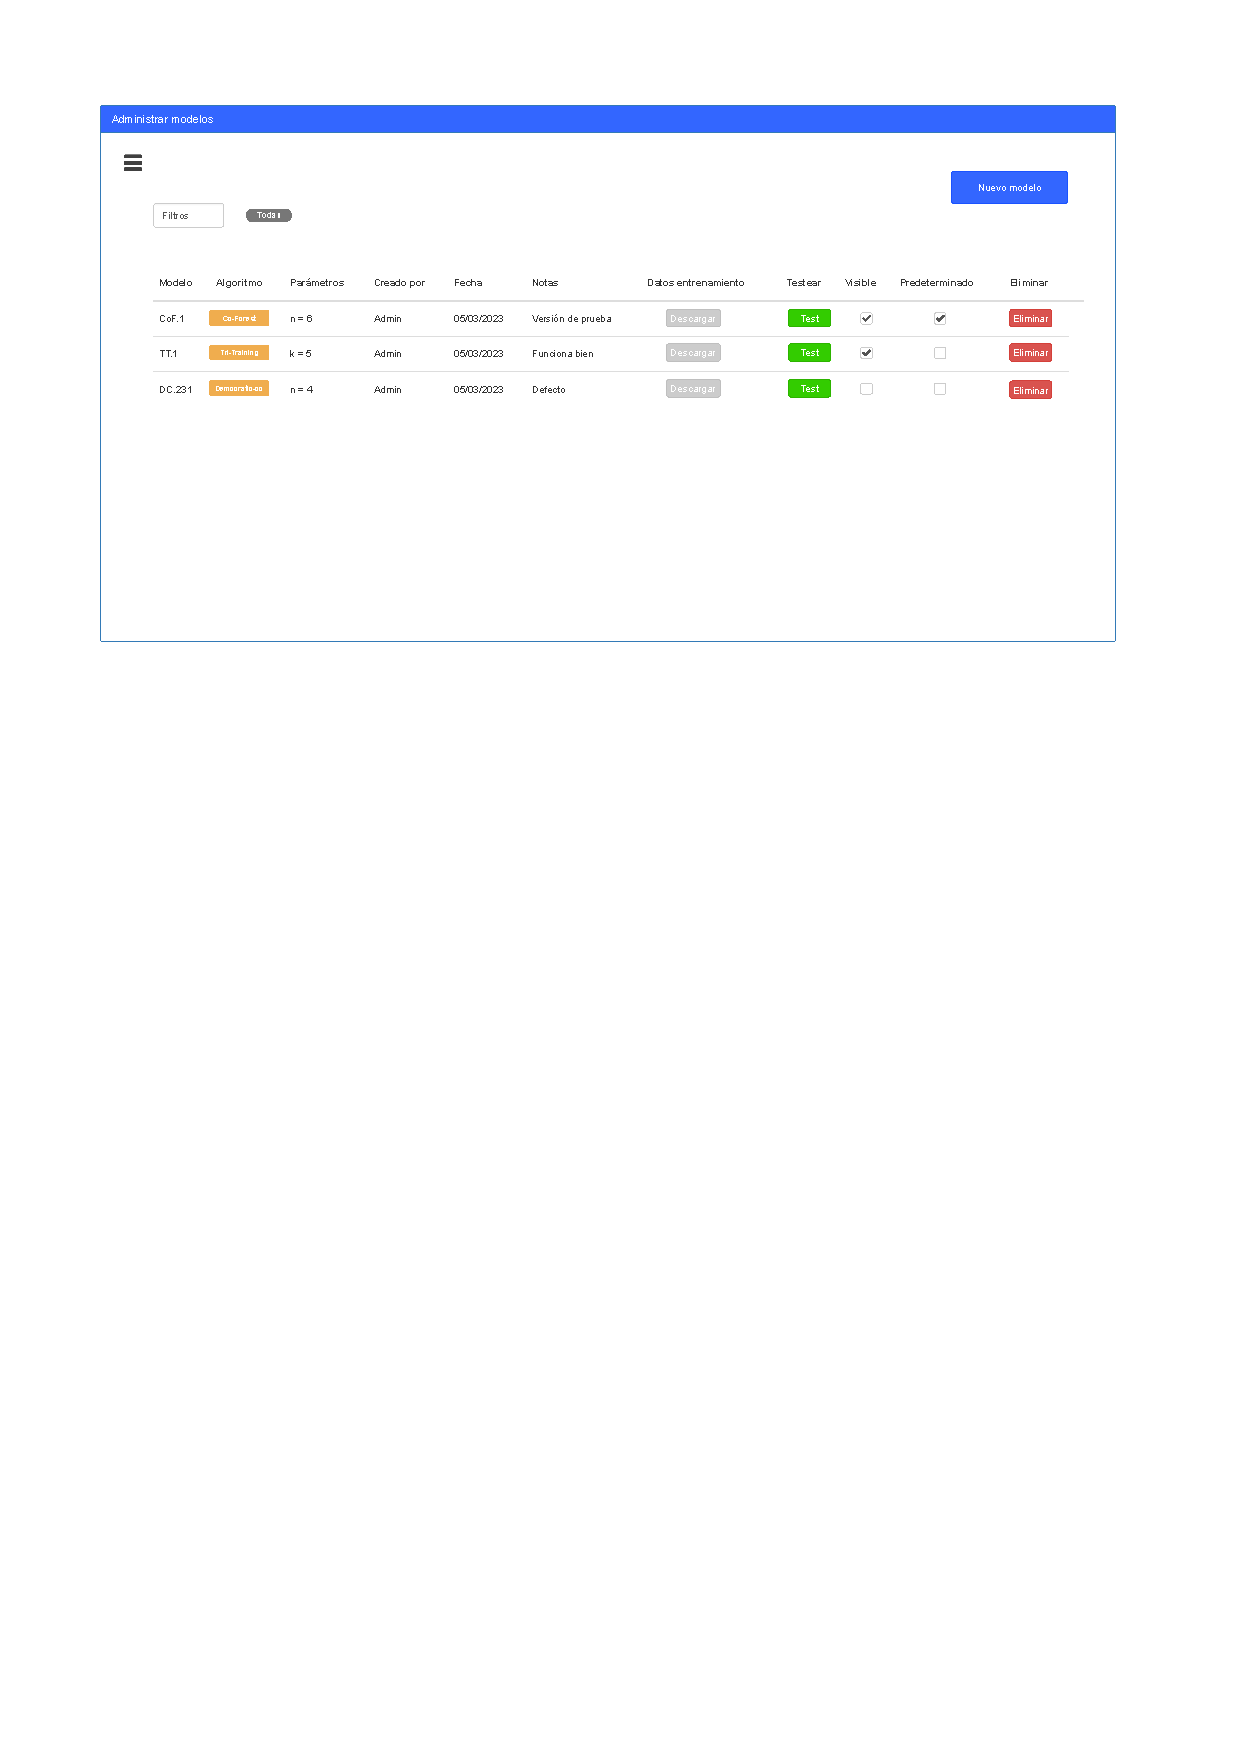
\includegraphics[width=\textwidth]{../img/anexos/mockups/5-mockups-models}
	\label{mock:model-admin}
\end{figure}

\begin{figure}[h]
	\caption{Prototipo: creación de modelos}
	\centering
	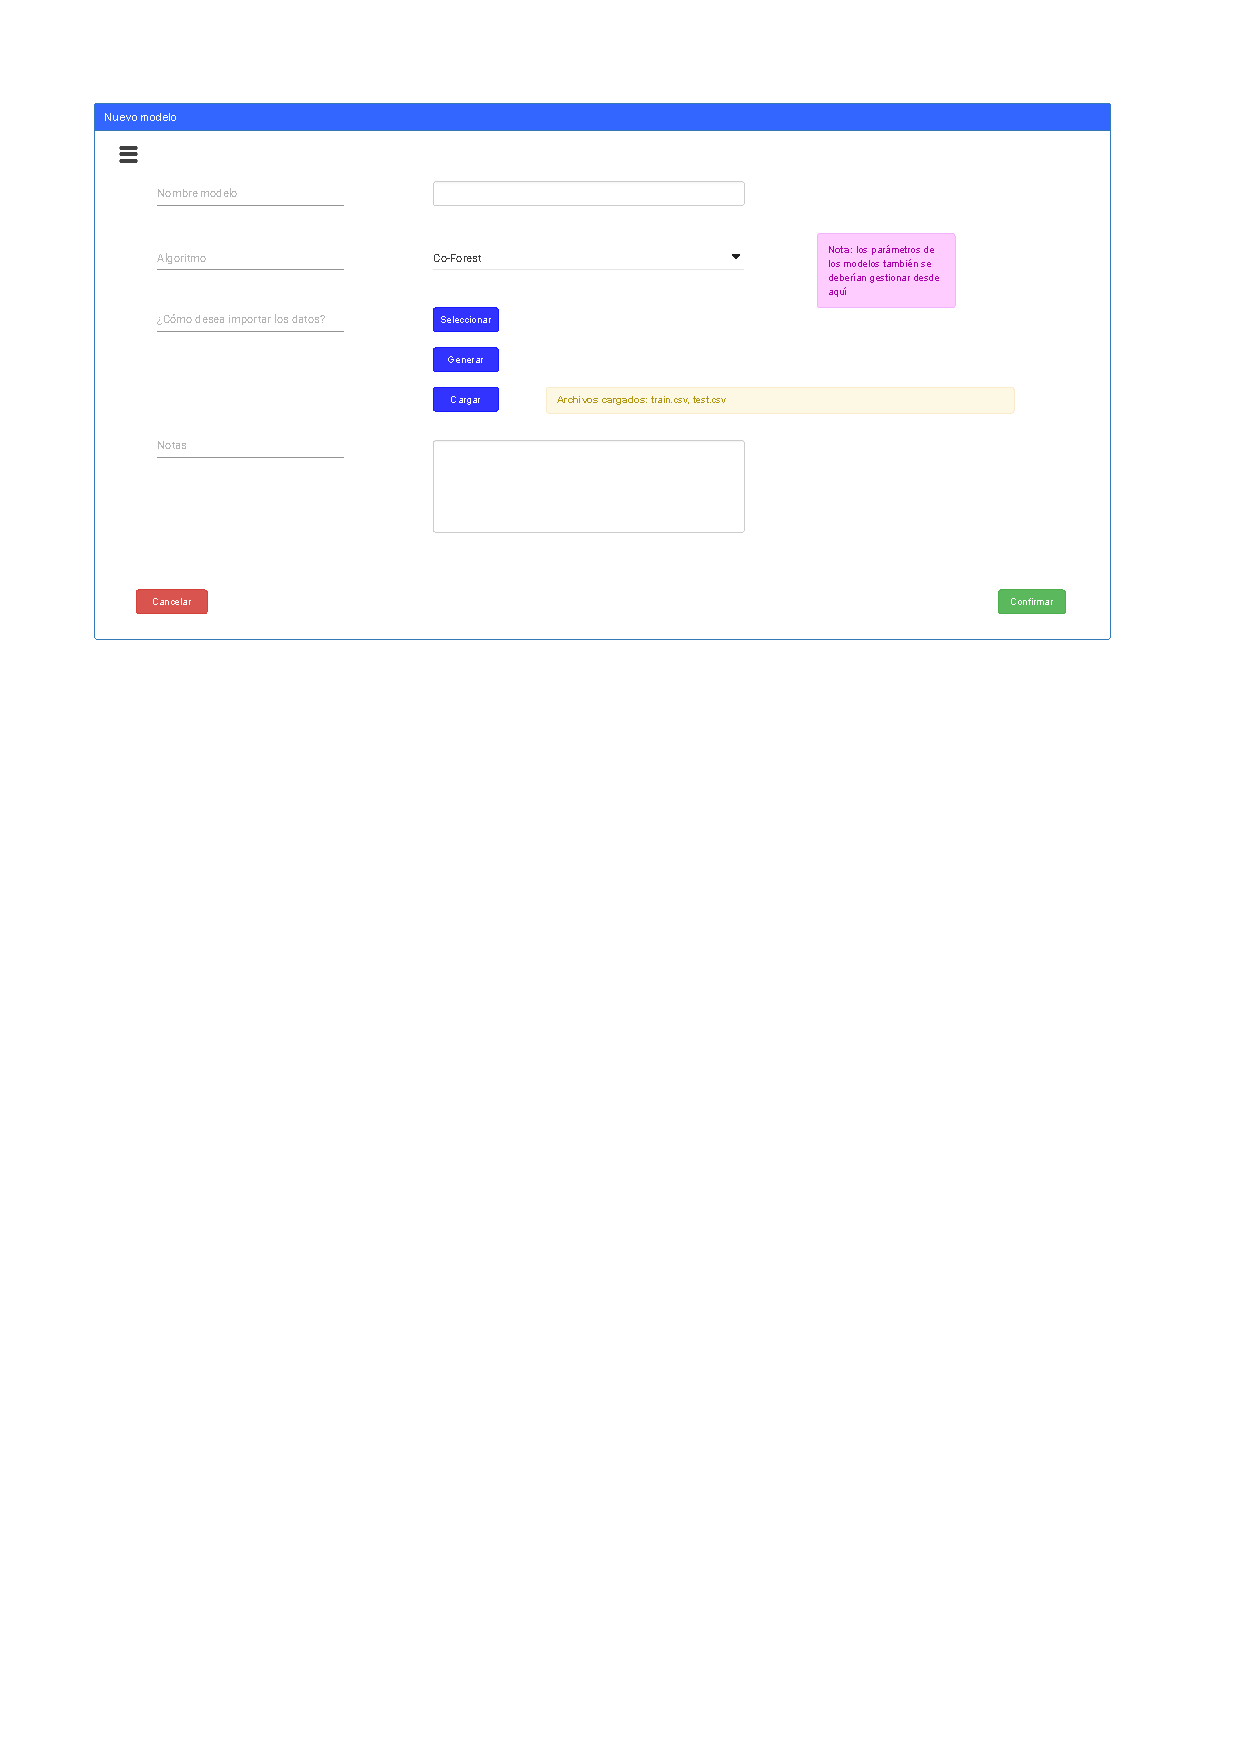
\includegraphics[width=\textwidth]{../img/anexos/mockups/6-mockups-new_model}
	\label{mock:model-new}
\end{figure}

\begin{figure}[h]
	\caption{Prototipo: evaluación de modelos}
	\centering
	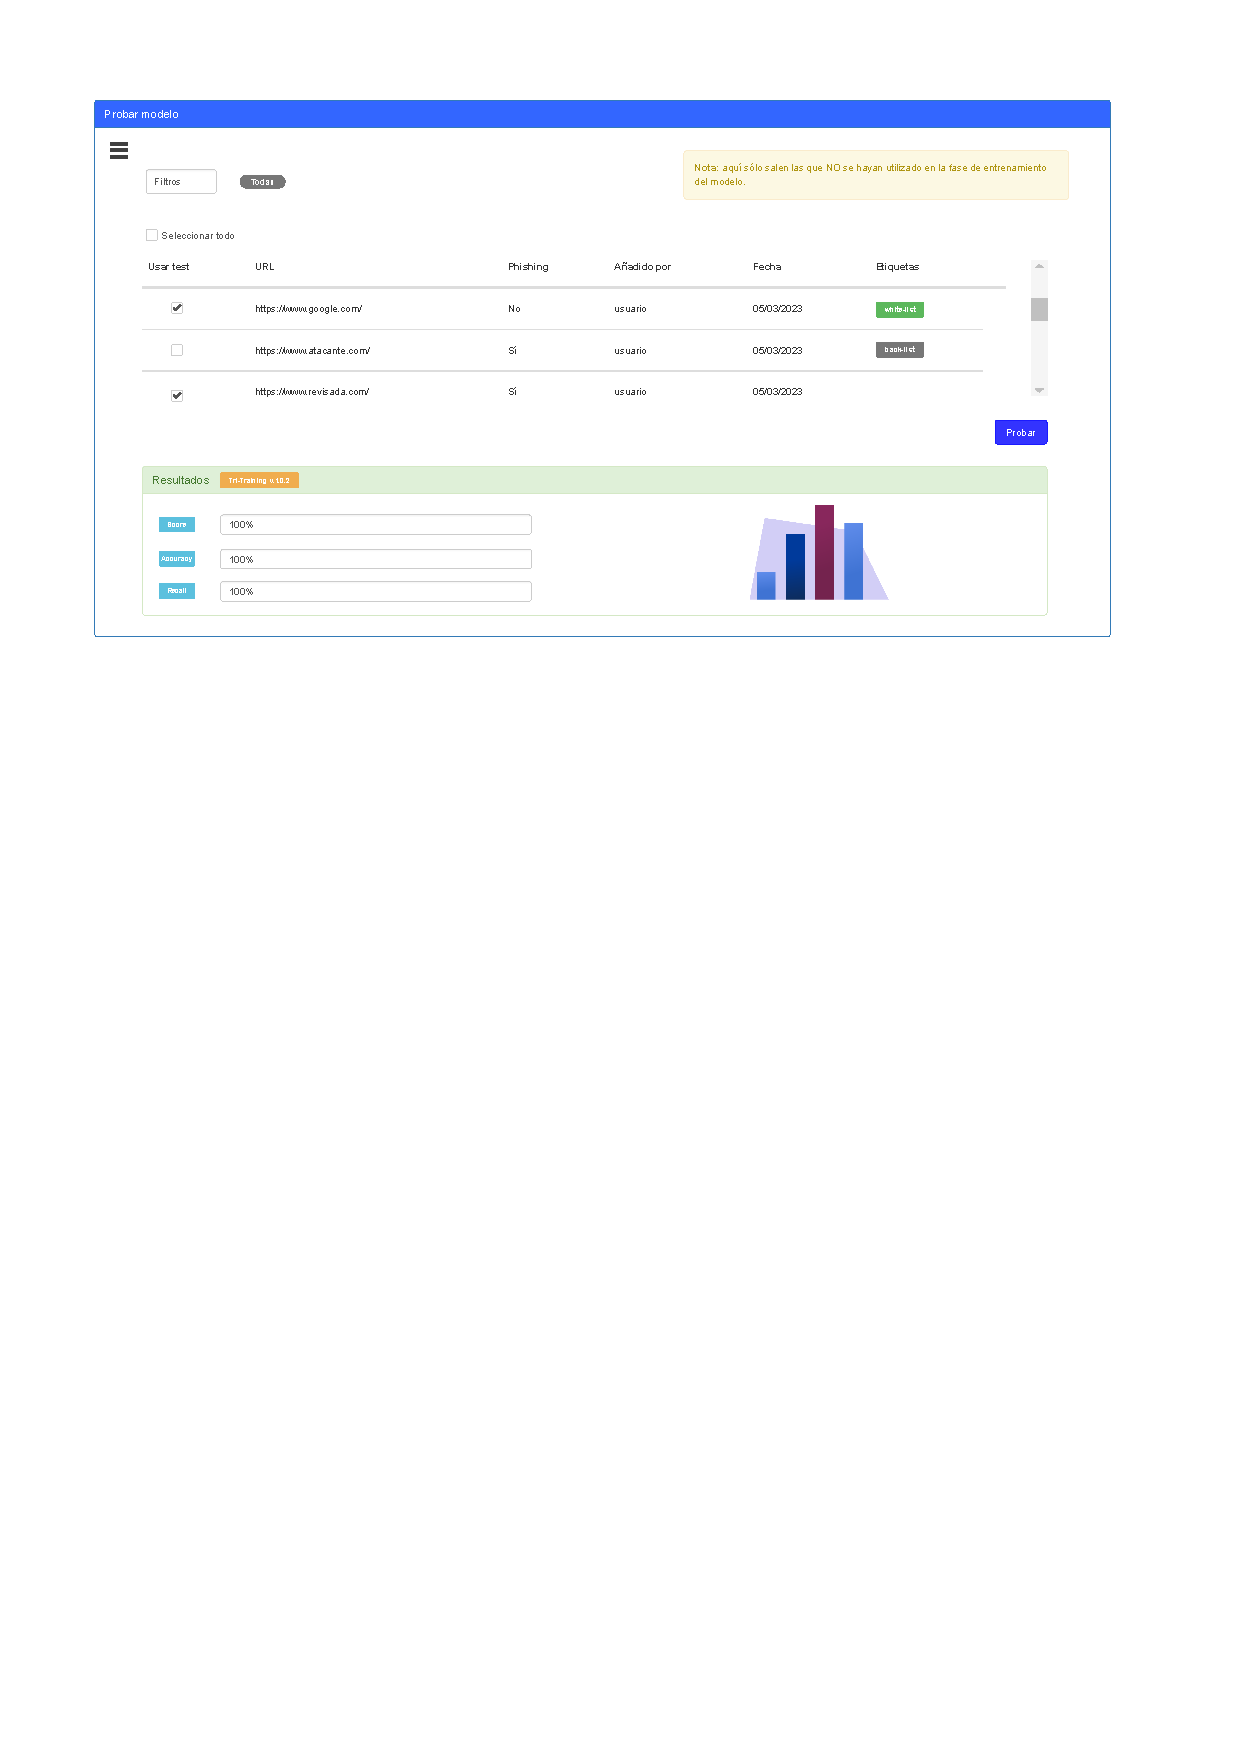
\includegraphics[width=\textwidth]{../img/anexos/mockups/7-mockups-test_model}
	\label{mock:model-test}
\end{figure}

\begin{figure}[h]
	\caption{Prototipo: selección de instancias}
	\centering
	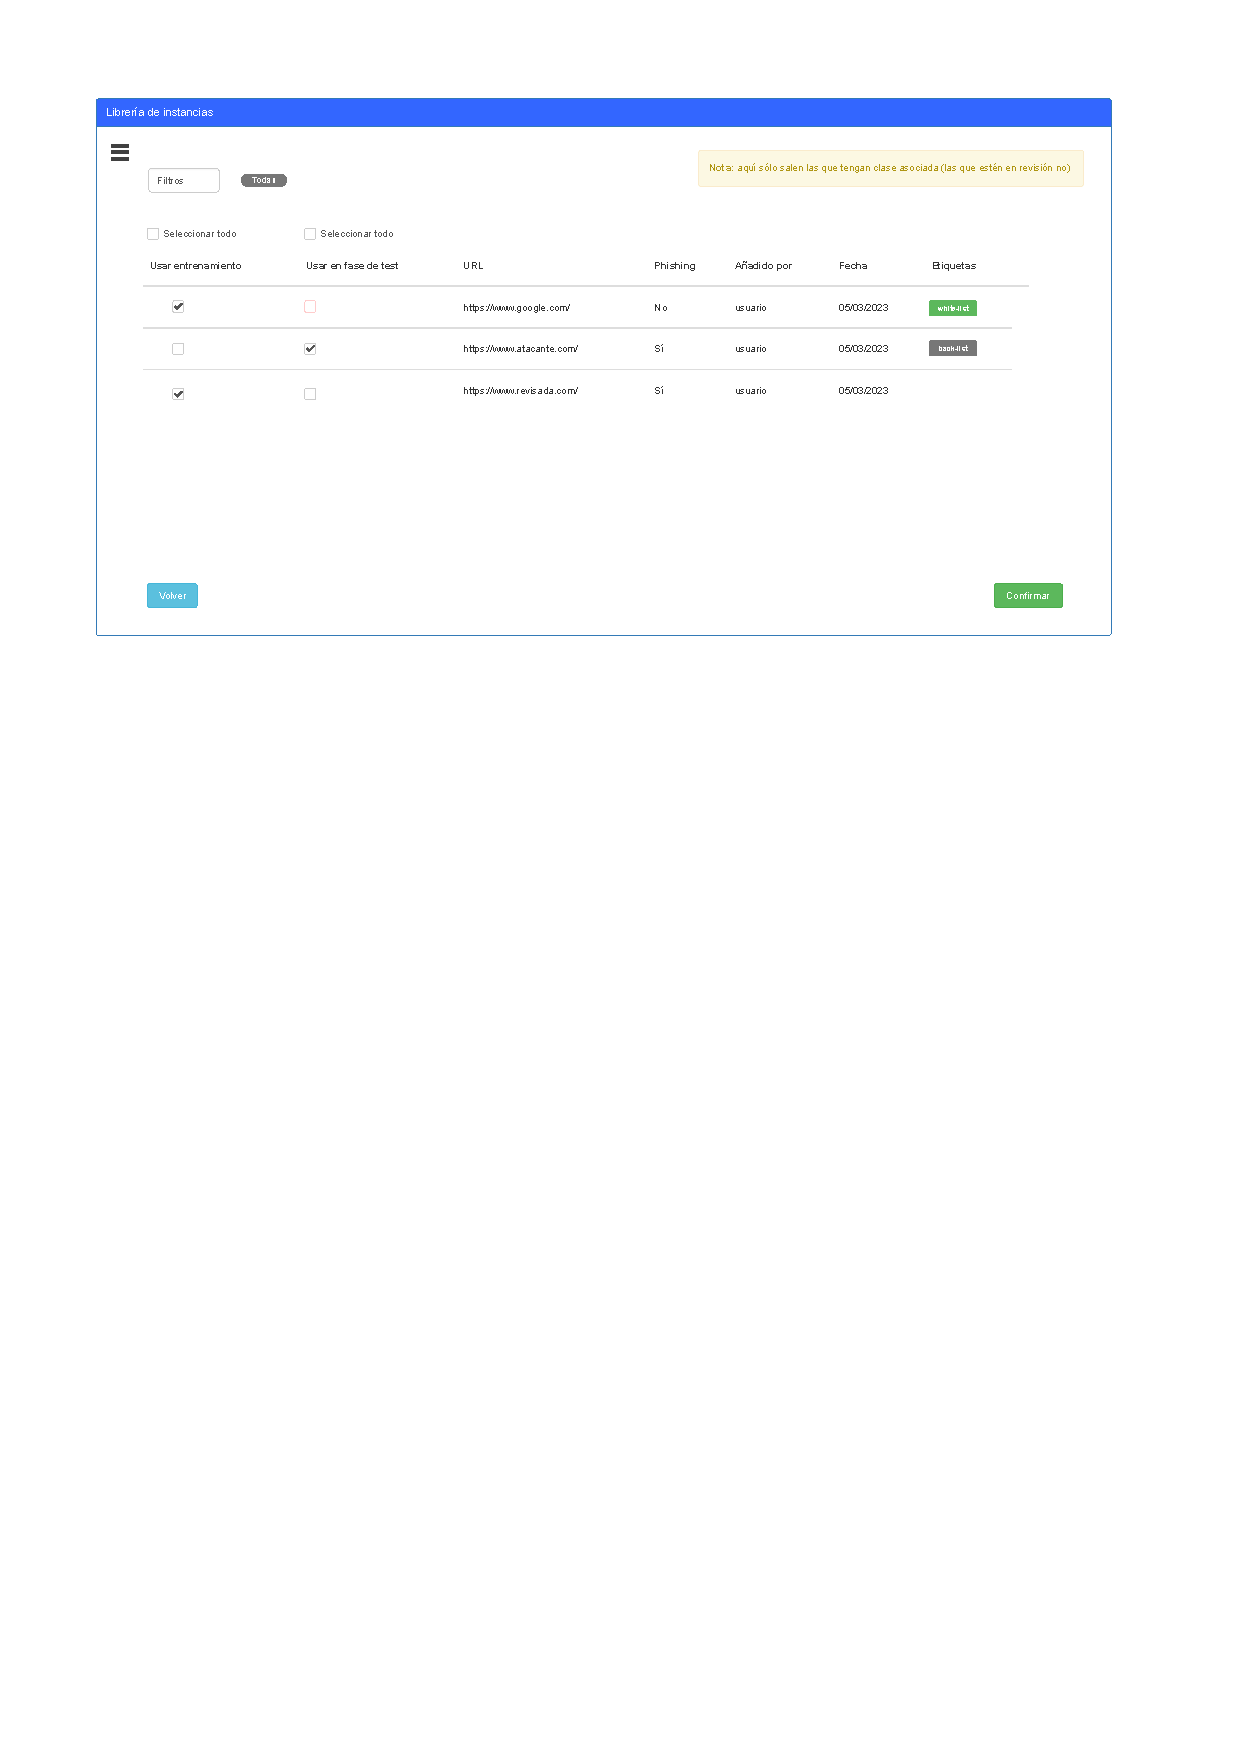
\includegraphics[width=\textwidth]{../img/anexos/mockups/8-mockups-select_instances}
	\label{mock:instance-selection}
\end{figure}

\begin{figure}[h]
	\caption{Prototipo: administración de instancias}
	\centering
	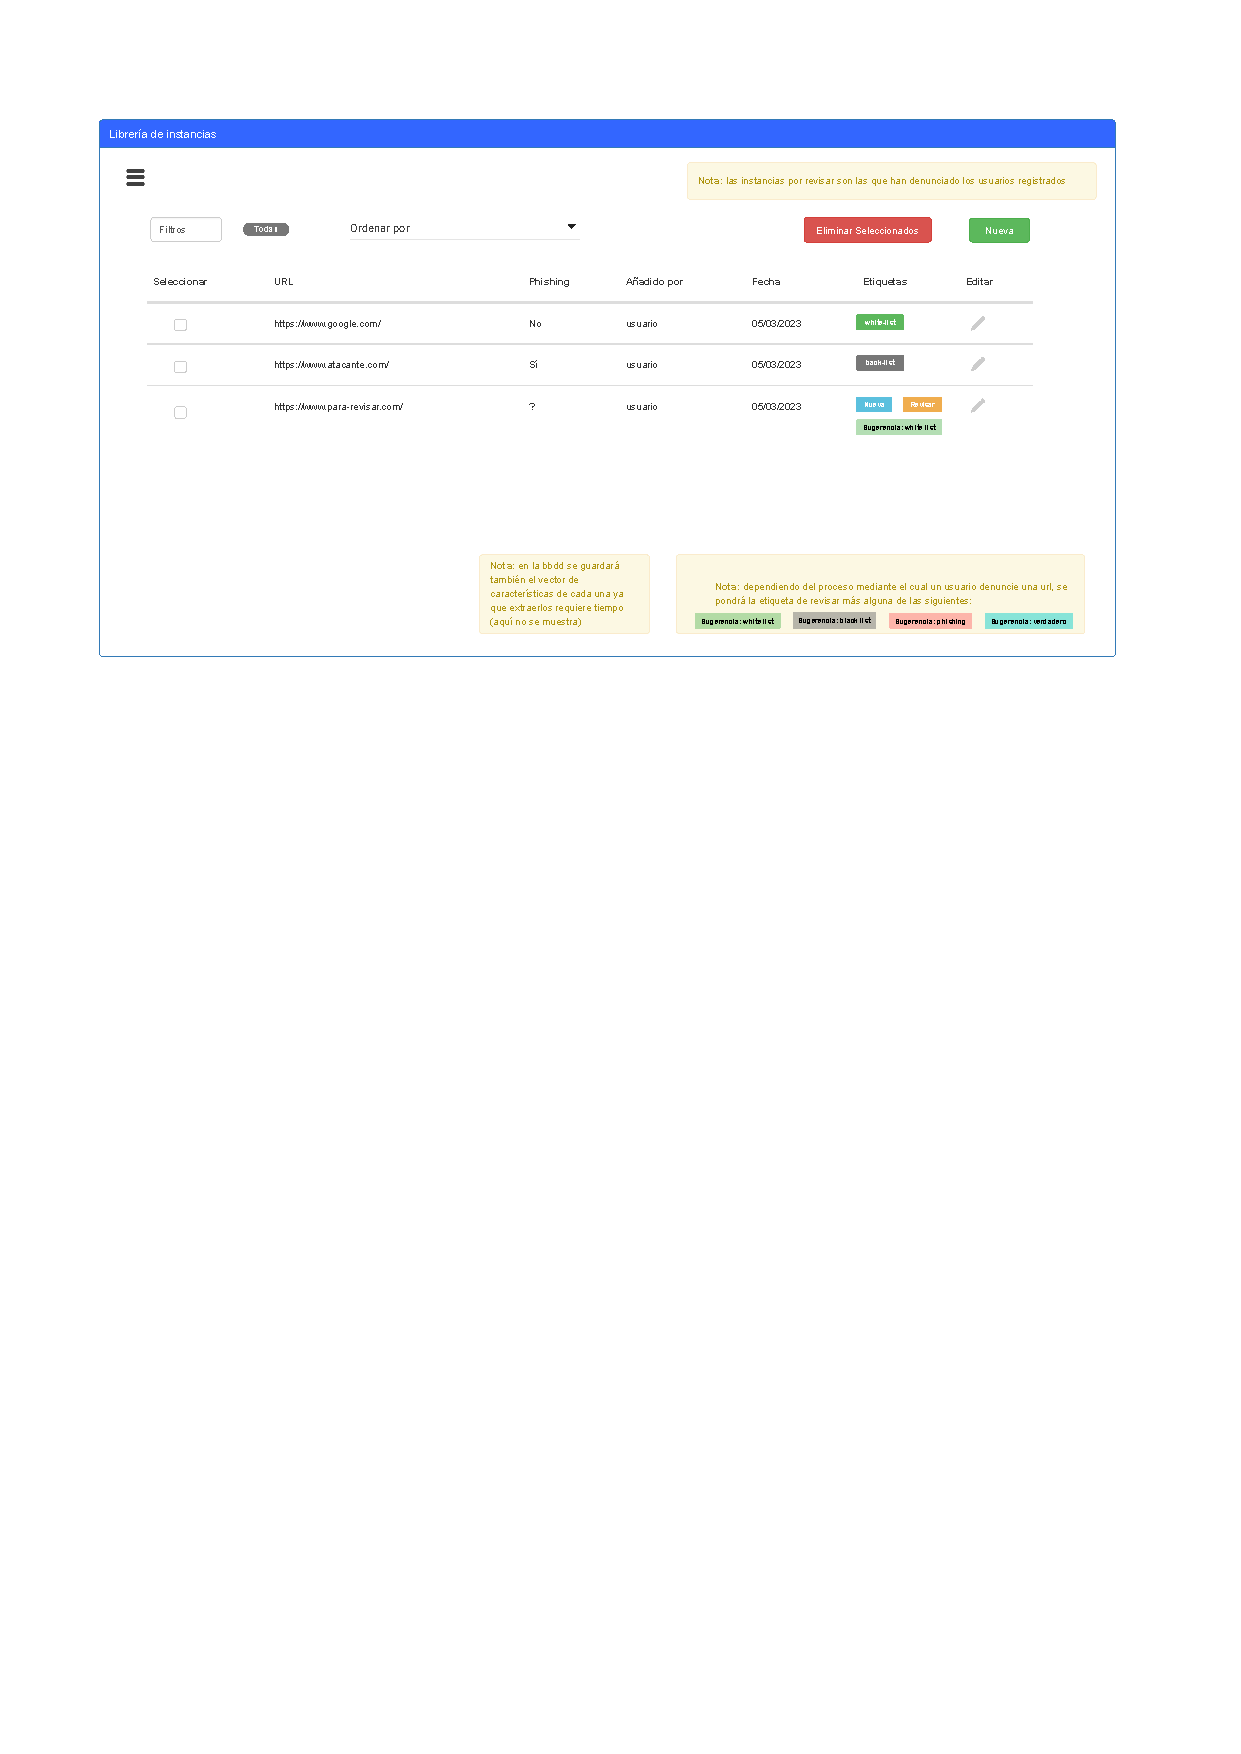
\includegraphics[width=\textwidth]{../img/anexos/mockups/9-mockups-instances}
	\label{mock:instance-admin}
\end{figure}

\begin{figure}[h]
	\caption{Prototipo: edición de instancias}
	\centering
	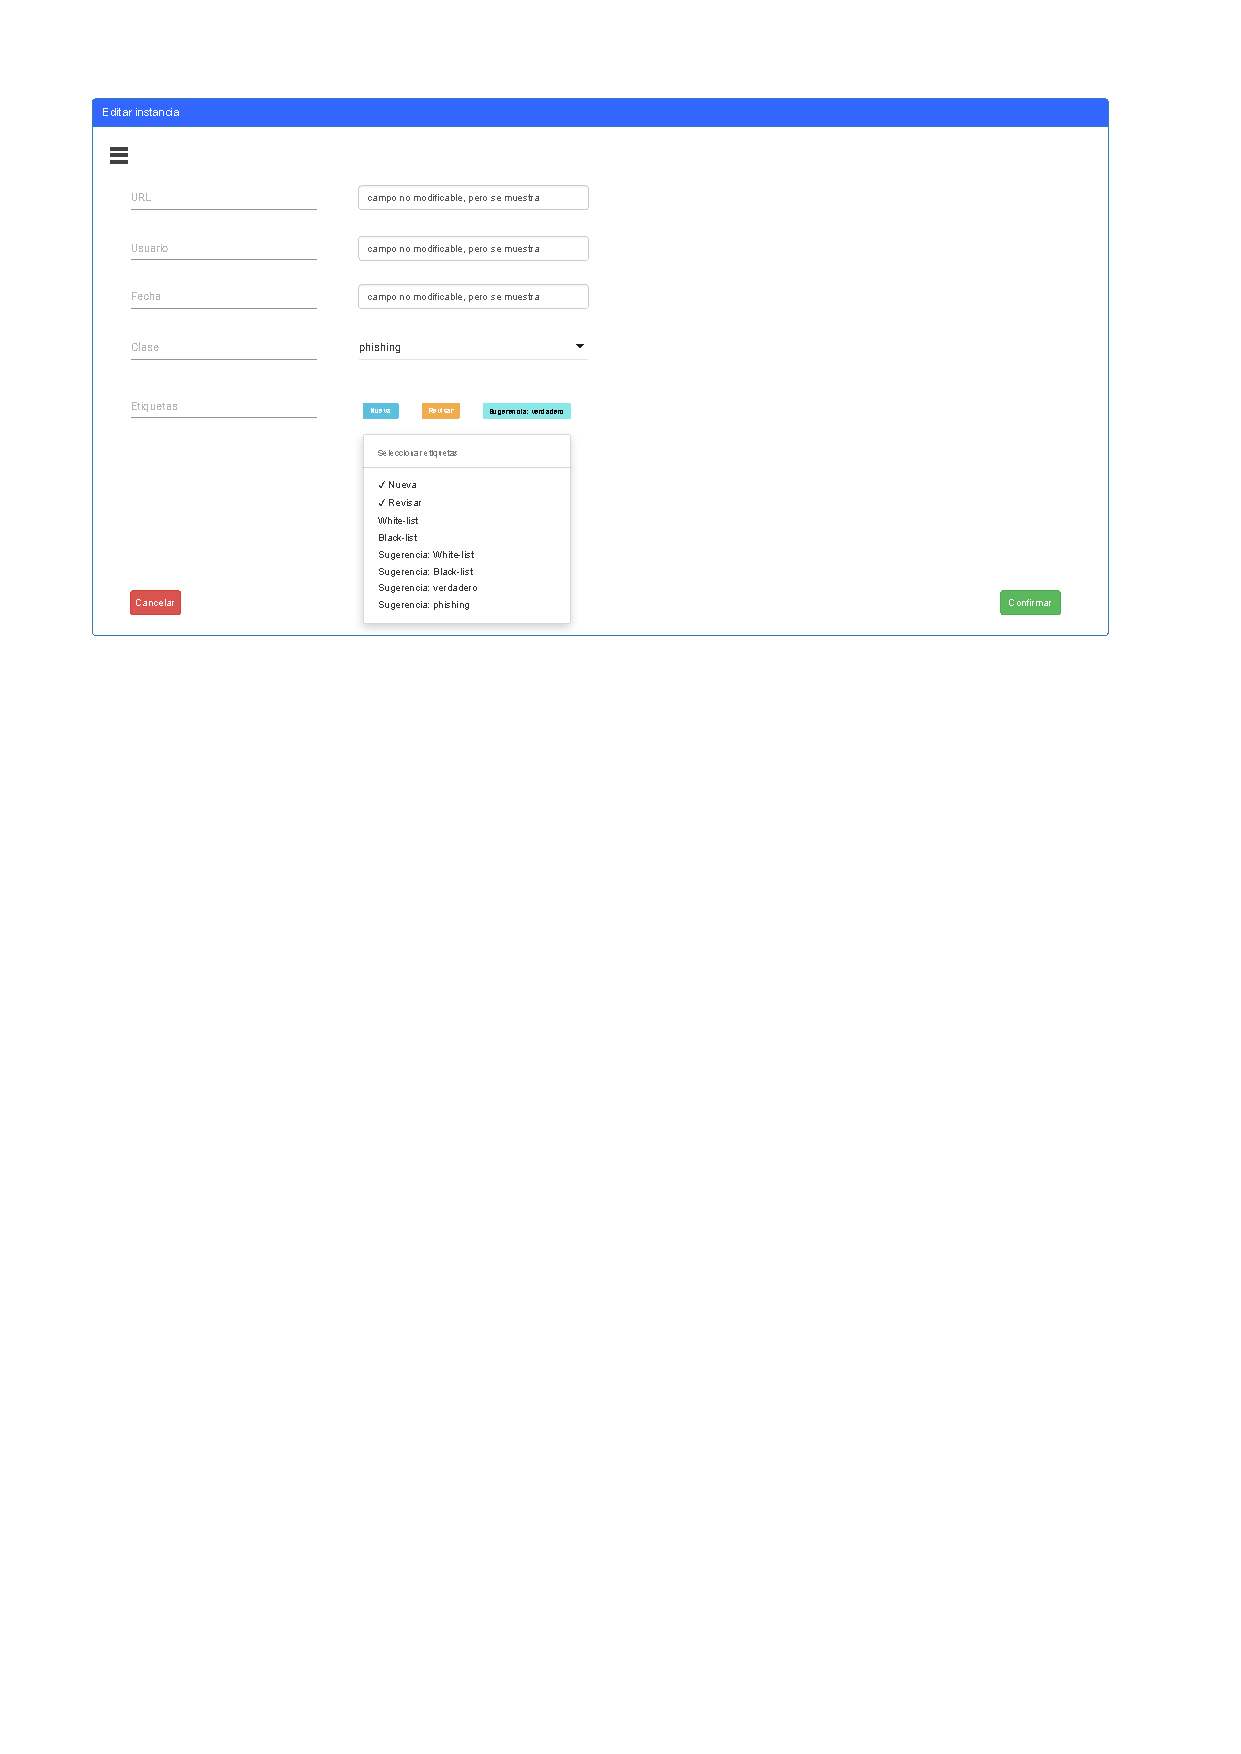
\includegraphics[width=\textwidth]{../img/anexos/mockups/10-mockups-edit_instance}
	\label{mock:instances-edit}
\end{figure}

\section{Catálogo de requisitos}
\label{s:cat-requisitos}

Utilizando como base las entrevistas realizadas con el \textit{product owner}, las historias de usuario expuestas en la sección~\ref{s:hu} y como soporte auxiliar los prototipos de la sección~\ref{s:mockups}, se han extraído los requisitos de usuario de forma tradicional y siguiendo las características que han de tener según el estándar~\texttt{IEEE 830}~\cite{ieee830}. Por ello, se dividen en dos categorías:

\subsection{Requisitos funcionales}
\label{s:requisitos-funcionales}

Este tipo de requerimiento (de ahora en adelante RF) detalla las funciones que debe realizar la pieza de \textit{software} desarrollada (en este caso, la página \textit{web}) para cumplir con las expectativas del usuario. Es decir, se centra en qué debe hacer el sistema y cómo. En esta categoría se encuentran:

\begin{itemize}
	\item \textbf{RF-1 Análisis de enlaces}: la página \textit{web} ha de ser capaz de analizar un enlace y concluir si se trata de un enlace de \textit{phishing} o legítimo mediante el uso de \textit{machine learning}\footnote{Una idea intuitiva de lo que desea el usuario se puede observar en el \textit{mockup}~\ref{mock:index}.}.
	\begin{itemize}
		\item \textbf{RF-1.1 Selección de modelos}: la página \textit{web} debe disponer de modelos entrenados para que el usuario pueda seleccionar los que desee para cada análisis.
		\item \textbf{RF-1.2 Análisis rápido}: en caso de haber realizado un análisis de un enlace repetido, la página \textit{web} debe mostrar los resultados inmediatamente (sin necesidad de recalcularlo).
	\end{itemize}
	
	\item \textbf{RF-2 Visualización de resultados}: los resultados del análisis se deben mostrar utilizando técnicas de representación visual para facilitar el entendimiento por parte de cualquier tipo de usuario\footnote{Una idea intuitiva de lo que desea el usuario se puede observar en el \textit{mockup}~\ref{mock:dashboard}.}.
	\begin{itemize}
	\item \textbf{RF-2.1 Gráficos interactivos}: la página \textit{web} debe mostrar gráficos con las estadísticas de los modelos seleccionados para el análisis y de los resultados del mismo. Estos gráficos deben permitir que el usuario interactúe con ellos seleccionando la información que desea representar.
	\item \textbf{RF-2.2 Tablas}: se han de mostrar tablas con información acerca de cada clasificador, qué predicción ha realizado y cómo de seguro está de ella.
	\item \textbf{RF-2.3 Vector de características}: se debe mostrar (y explicar) de dónde proviene el resultado extraído y cómo se ha calculado.
	\item \textbf{RF-2.4 Notificar falso resultado}: en caso de que un usuario registrado piense que un análisis es incorrecto, debe poder notificarlo fácilmente.
	\end{itemize}

	\item \textbf{RF-3 Usuarios}: se ha de incluir una gestión básica de usuarios con el fin de trazar quién ha realizado reportes de enlaces y moderar accesos a zonas restringidas.
	\begin{itemize}
	\item \textbf{RF-3.1 Creación de cuentas}: cualquier usuario visitante podrá crear una cuenta proporcionando un nombre de usuario, un \textit{email} y una contraseña.
	\item \textbf{RF-3.2 Inicio de sesión}: un usuario registrado podrá iniciar sesión en la página \textit{web} con sus credenciales.
	\item \textbf{RF-3.3 Visualización del perfil}: cualquier usuario registrado podrá consultar sus datos\footnote{Una idea intuitiva de lo que desea el usuario se puede observar en el \textit{mockup}~\ref{mock:profile}.}.
	\end{itemize}

	\item \textbf{RF-4 Reportar enlaces}: se permitirá que los usuarios registrados puedan reportar aquellos enlaces que sepan que son \textit{phishing} o legítimos. Estos serán etiquetados como pertenecientes a una lista blanca o a una lista negra y serán revisados por un administrador\footnote{Una idea intuitiva de lo que desea el usuario se puede observar en el \textit{mockup}~\ref{mock:report_url}.}.
	
	\item \textbf{RF-5 Administración de instancias:} una instancia es una URL de la que se desea almacenar información (como su vector de características, etiqueta, pertenencia a una lista blanca o negra, etc.)\footnote{Una idea intuitiva de lo que desea el usuario se puede observar en los \textit{mockups}~\ref{mock:instance-admin}, \ref{mock:instance-selection} y \ref{mock:instances-edit}.}.
	\begin{itemize}
		\item \textbf{RF-5.1 Creación de instancias}: se deberán de poder añadir instancias\footnote{En el contexto de este proyecto, una instancia es cada uno de los datos que puede ser utilizado para entrenar o probar un modelo (URLs que serán clasificadas como \textit{phishing} o legítimas).}  a la base de datos.
		\item \textbf{RF-5.2 Modificación de instancias}: se podrán editar ciertos campos relacionados con cada instancia (como sus etiquetas o pertenencia a listas). Además, se debe permitir que los usuarios puedan regenerar vectores de características desde la aplicación.
		\item \textbf{RF-5.3 Eliminación de instancias}: se podrán borrar enlaces del \textit{dataset}.
		\item \textbf{RF-5.4 Descarga de instancias}: se podrán descargar las instancias seleccionadas en un archivo \texttt{csv} para ser utilizadas en el entrenamiento o prueba de nuevos modelos.
	\end{itemize}
	
	\item \textbf{RF-6 Administración de modelos}: un administrador debe poder gestionar desde la aplicación los modelos de aprendizaje disponibles para analizar enlaces\footnote{Una idea intuitiva de lo que desea el usuario se puede observar en los \textit{mockups}~\ref{mock:model-admin}, \ref{mock:model-new} y \ref{mock:model-test}.}.
	\begin{itemize}
	\item \textbf{RF-6.1 Creación de modelos}: se deberá poder crear nuevos modelos de aprendizaje que estarán disponibles para ser utilizados por los usuarios de la web.
	\begin{itemize}
		\item \textbf{RF-6.1.1 Parámetros generales}: el administrador podrá personalizar todos los atributos que desee tales como el nombre del clasificador, su versión, su semilla aleatoria, las notas, etc. Además, también podrá definir dos atributos fundamentales:
		\begin{enumerate}
			\item Visibilidad: un modelo visible está disponible para ser usado en la página web.
			\item Clasificador por defecto: un modelo que sea el clasificador por defecto será el utilizado cuando un usuario realice un análisis y no seleccione ningún modelo para analizar.
		\end{enumerate}
		\item \textbf{RF-6.1.2 Selección del algoritmo}: el administrador podrá seleccionar cualquiera de los siguientes algoritmos de aprendizaje semisupervisado: \textit{co-forest}, \textit{tri-training} o \textit{democratic-co learning}. Además, podrá personalizar los parámetros propios de cada uno.
		\item \textbf{RF-6.1.3 Selección del conjunto de datos de entrenamiento}: se podrá decidir con qué instancias se entrena el \textit{ensemble}. Para ello se podrán subir ficheros \texttt{.csv}.
		\item \textbf{RF-6.1.4 Selección del conjunto de datos de \textit{test}}: se podrá decidir con qué datos se realiza una primera evaluación del modelo creado. Para ello se podrán subir ficheros \texttt{.csv}.
	\end{itemize}
	
	\item \textbf{RF-6.2 Modificación de modelos}: se podrán editar ciertos campos de los modelos creados, como su visibilidad o su valor por defecto. No se podrán reentrenar modelos (son inmutables).
	\item \textbf{RF-6.3 Eliminación de modelos}: se podrán borrar modelos y dejarán de estar disponibles en el sistema.
	\item \textbf{RF-6.4 Evaluación de modelos}: se podrán evaluar fiablemente modelos previamente creados para actualizar las estadísticas que se muestran en los gráficos y visualizar sus rendimientos.
	\end{itemize}


	\item \textbf{RF-7 Administración de sugerencias}: un administrador debe poder gestionar desde la aplicación los reportes o las notificaciones del resto de usuarios.
\begin{itemize}
	\item \textbf{RF-7.1 Aceptar sugerencia}: se deberán poder aceptar las sugerencias que hayan hecho los usuarios y los resultados se reflejarán en las instancias afectadas.
	
	\item \textbf{RF-7.2 Descartar sugerencias}: se podrán descartar las sugerencias que se consideren inapropiadas.
\end{itemize}

\end{itemize}

\subsection{Requisitos no funcionales}
\label{s:requisitos-no-funcionales}

Por otro lado, estos requisitos (de ahora en adelante RNF) se centran en aspectos no relacionados con la operatividad del sistema. Es decir, están enfocados a describir cómo debe funcionar y no en la funcionalidad. Algunos ejemplos son:


\begin{itemize}
	\item \textbf{RNF-1 Seguridad}: el sistema debe proteger la información sensible de los usuarios.
	\begin{itemize}
		\item \textbf{RNF-1.1 Protección de credenciales}: todas las contraseñas han de estar correctamente cifradas y almacenadas en la base de datos.
		\item \textbf{RNF-1.2 Protección anti-rastreo}: las llamadas a sitios no seguros se deben realizar utilizando \textit{proxies} que oculten la dirección IP de los usuarios.
		\item \textbf{RNF-1.3 Control de acceso}: los usuarios que intenten acceder a páginas para las que no estén autorizados deben de ser redirigidos fuera de ellas.
	\end{itemize}
	\item \textbf{RNF-2 Usabilidad}: el \textit{software} desarrollado debe ser intuitivo y accesible para todos los usuarios.
	\begin{itemize}
		\item \textbf{RNF-2.1 Interfaces}: las interfaces han de estar diseñadas para facilitar las tareas y que se realicen en el menor tiempo posible. Además, han de ser agradables (inclusión de imágenes).
		\item \textbf{RNF-2.2 Tratamiento de excepciones}: en caso de ocurrir una situación imprevista, el usuario ha de ser redirigido a una página segura y correctamente informado mediante un mensaje entendible, significativo y transparente de lo ocurrido.
	\end{itemize}
	\item \textbf{RNF-3 Disponibilidad}: el sistema debe estar disponible para los usuarios y recuperarse rápidamente en caso de fallo.
	\item \textbf{RNF-4 Interoperabilidad}: el software desarrollado debe ser compatible con diversos sistemas y plataformas. Por este motivo, se ha optado por una \textit{web}.
	\item \textbf{RNF-5 Mantenibilidad}: el \textit{software} desarrollado ha de estar correctamente documentado, refactorizado y analizado para facilitar la inclusión de nuevos desarrolladores y la corrección del mismo.
	\item \textbf{RNF-6 Escalabilidad}: la plataforma desarrollada debe manejar un alto número de usuarios sin afectar su rendimiento.
	\item \textbf{RNF-7 Rendimiento}: el sistema debe tener un tiempo de respuesta adecuado incluso bajo situaciones de alta carga. En caso de relizar operaciones que requieran esperas largas por parte del usuario, se ha de informar y amenizar dicha espera mediante el uso de pantallas interactivas.
	\item \textbf{RNF-8 Internacionalización}: la página ha de estar disponible en más de un idioma.
	\item \textbf{RNF-9 Soporte}: el equipo de desarrollo debe poder ser contactado por \textit{email} o GitHub y permitir la notificación de \textit{bugs}, ideas de nueva funcionalidad o consultas acerca de la aplicación.
	\item \textbf{RNF-10 Exactitud}: el sistema debe de ser capaz de caracterizar fielmente las características de una página legítima o de \textit{phishing} y debe distinguir ambos casos con facilidad.
\end{itemize}

\section{Especificación de requisitos}
\label{s:requisitos}

Se detalla a continuación la especificación de requisitos tradicional de la aplicación \textit{web} propuesta basada en el catálogo de requisitos de la sección~\ref{s:cat-requisitos}.

\subsection{Diagrama de casos de uso}
\label{ss:diagrama-casos-uso}

Partiendo de las historias de usuario extraídas en las entrevistas realizadas con el \textit{product owner} y de los \textit{mockups} mostrados en la sección~\ref{s:mockups}, se ha extraído el diagrama de casos de uso disponible en la figura~\ref{b:diagrama-cu}. A continuación de este diagrama, se muestran las tablas correspondientes a cada caso de uso.

\begin{figure}[h]
	\caption[Diagrama: casos de uso]{Diagrama general de casos de uso de la aplicación.}
	\centering
	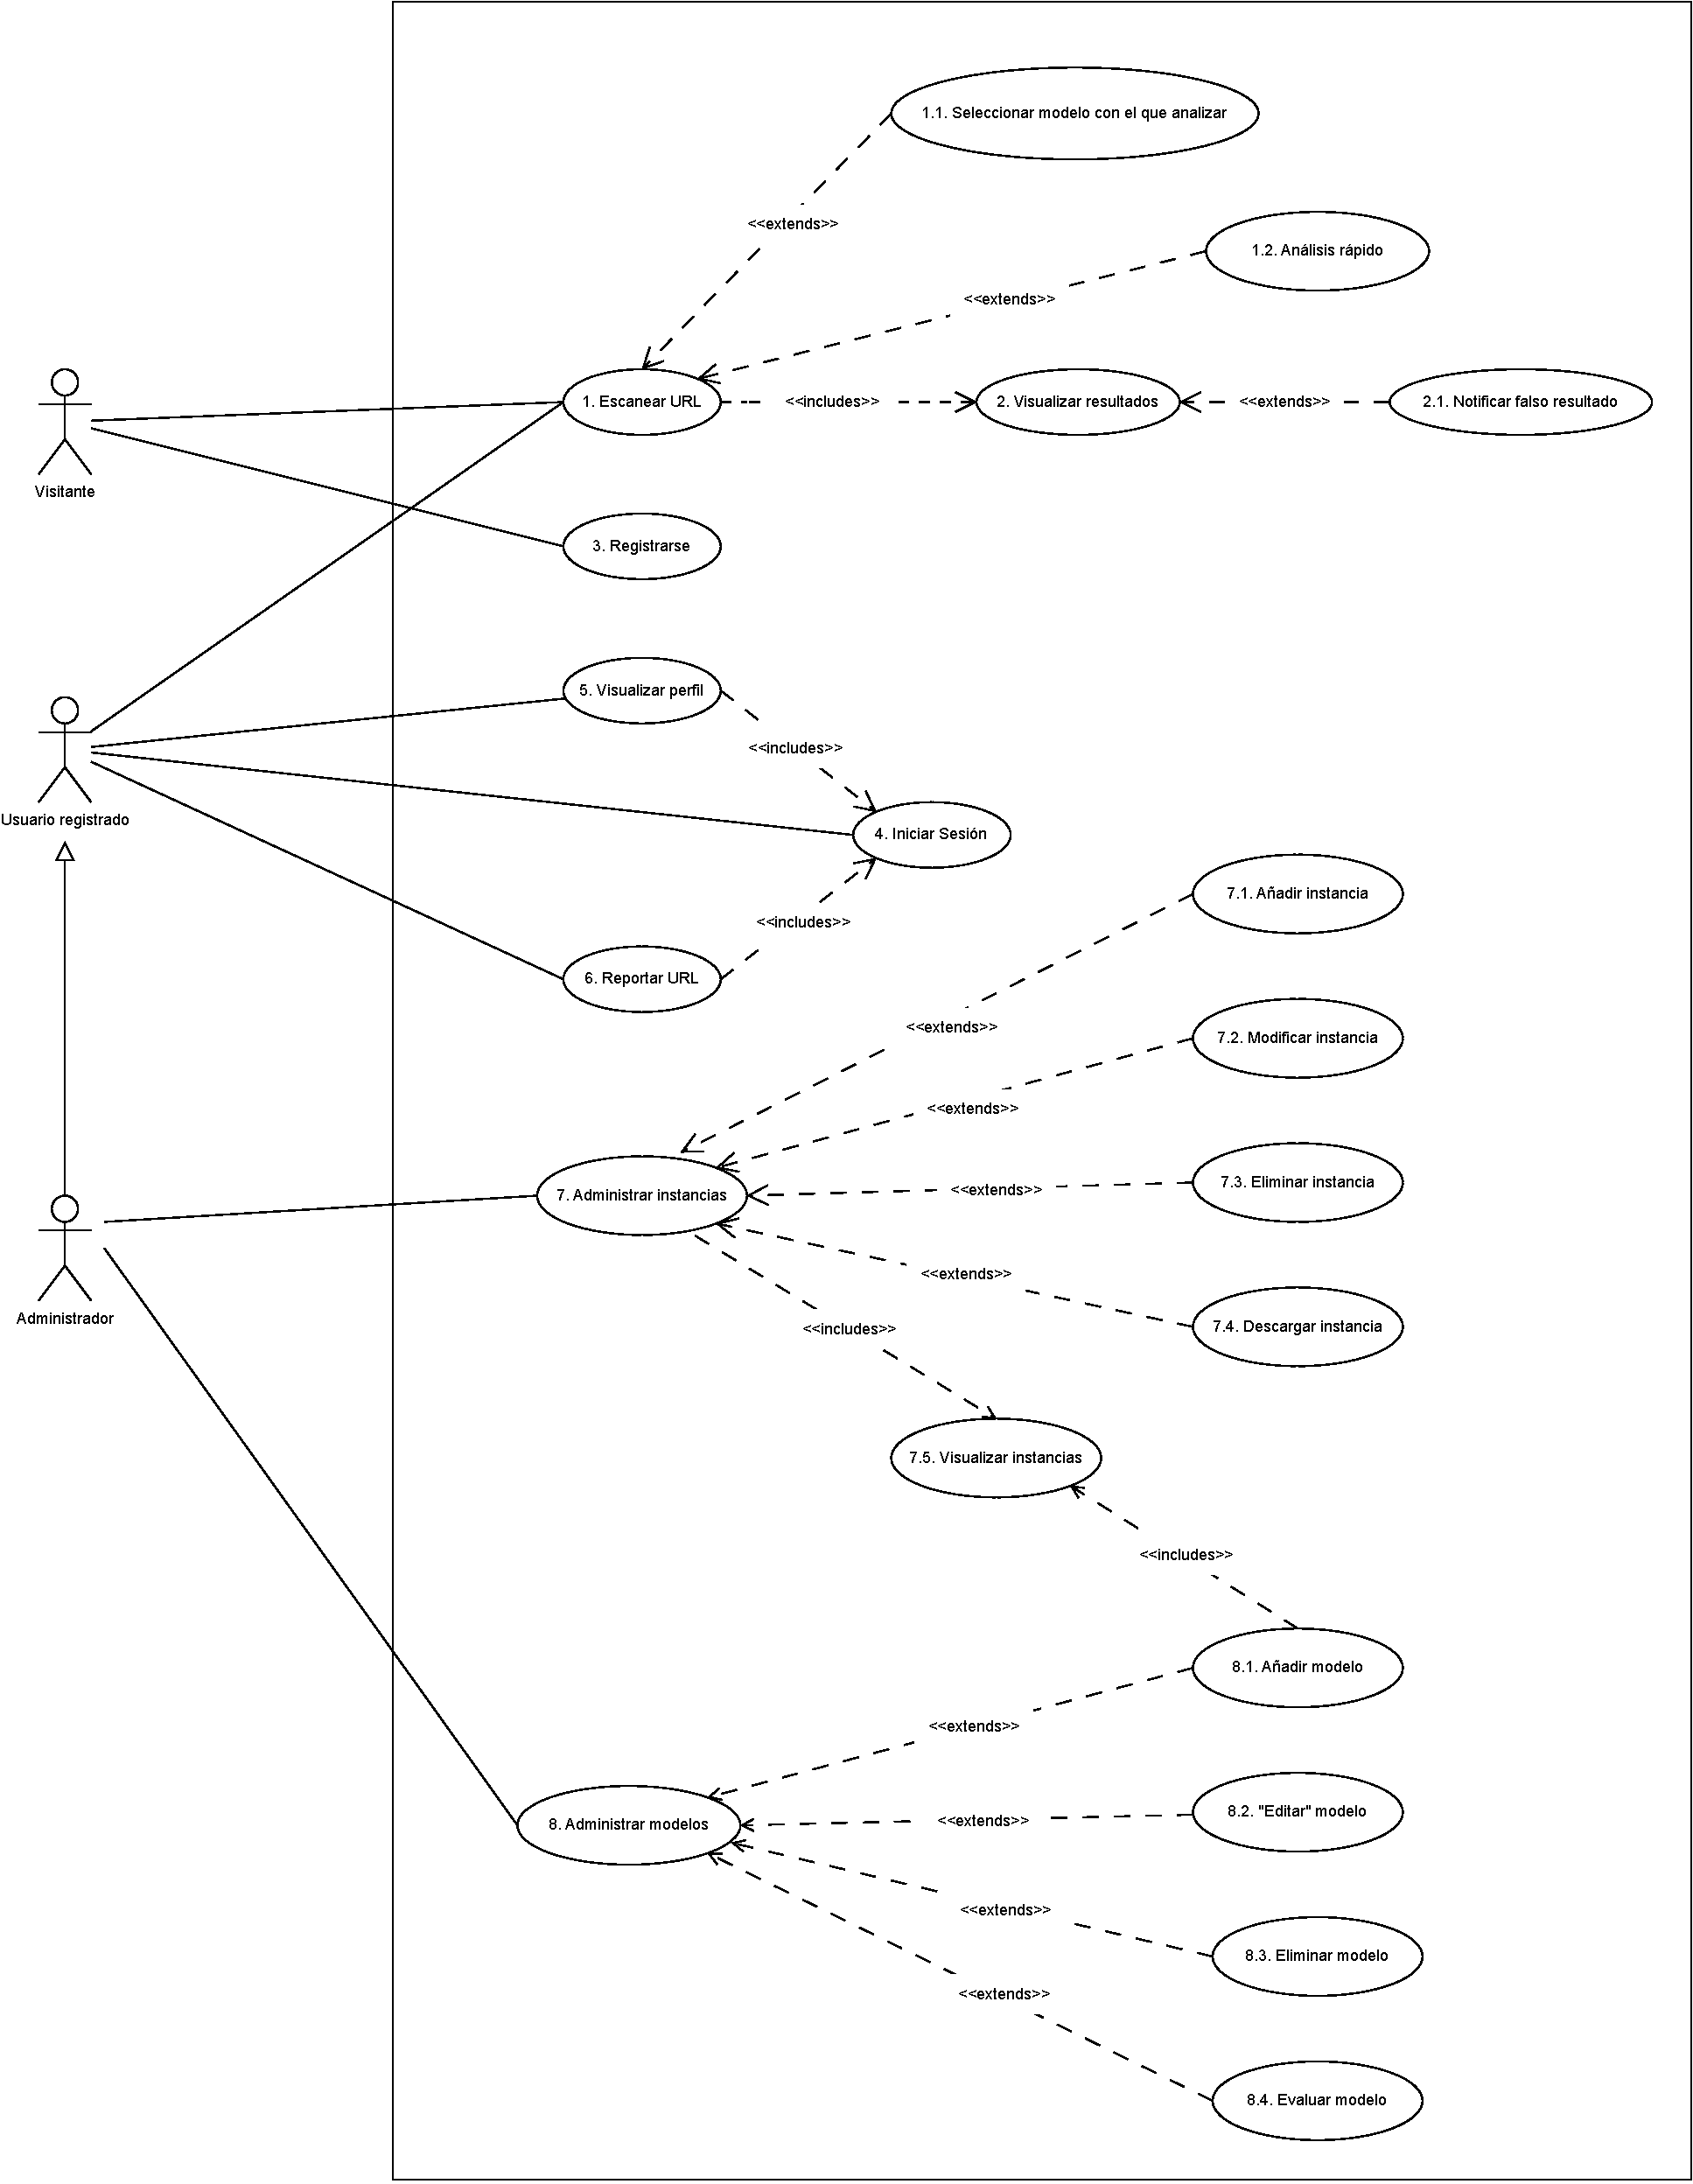
\includegraphics[width=\textwidth]{../img/anexos/diagrams/cu}
	\label{b:diagrama-cu}
\end{figure}

% Caso de Uso 1 -> Escanear URL
\begin{table}[p]
	\centering
	\begin{tabularx}{\linewidth}{ p{0.21\columnwidth} p{0.71\columnwidth} }
		\toprule
		\textbf{CU-1}    & \textbf{Escanear URL}\\
		\toprule
		\textbf{Versión}              & 1.0    \\
		\textbf{Autor}                & Patricia Hernando Fernández \\
		\textbf{Requisitos asociados} & RF-1 (RF-1.1, RF-1.2) \\
		\textbf{Descripción}          & Permitir que un usuario realice un escaneo de la URL que desee. Para ello, seleccionará los modelos que considere adecuados y se mostrarán los resultados en un \textit{dashboard} (CU-2 en la tabla~\ref{cu:visualizar-resultados}). \\
		\textbf{Precondición}         & No hay precondiciones. \\
		\textbf{Acciones}             &
		\begin{enumerate}
			\def\labelenumi{\arabic{enumi}.}
			\tightlist
			\item El usuario introduce la URL.
			\item El usuario selecciona los modelos de ML que considere (consultar CU-1.1 en la tabla~\ref{cu:seleccionar-modelos-ml}).
			\item El usuario decide si quiere realizar un análisis rápido (consultar CU-1.2 en la tabla~\ref{cu:analisis-rapido}).
			\item El usuario pulsa el botón de <<realizar análisis>>.
		\end{enumerate}\\
		\textbf{Postcondición}        & No hay postcondiciones. \\
		\textbf{Excepciones}          & En caso de que la URL introducida sea inalcanzable (tras aplicar reintentos) o que no haya ningún modelo disponible, el usuario será notificado y redirigido a la página principal. \\
		\textbf{Importancia}          & Alta \\
		\bottomrule
	\end{tabularx}
	\caption{CU-1 Escanear URL.}
	\label{cu:escanear-url}
\end{table}


% Caso de Uso 1.1 -> Seleccionar modelos
\begin{table}[p]
	\centering
	\begin{tabularx}{\linewidth}{ p{0.21\columnwidth} p{0.71\columnwidth} }
		\toprule
		\textbf{CU-1.1}    & \textbf{Seleccionar modelos con los que analizar}\\
		\toprule
		\textbf{Versión}              & 2.0    \\
		\textbf{Autor}                & Patricia Hernando Fernández \\
		\textbf{Requisitos asociados} & RF-1.1 \\
		\textbf{Descripción}          & Se mostrará al usuario los distintos modelos disponibles (y visibles) para que elija los que desee. \\
		\textbf{Precondición}         & Estar realizando el CU-1 (disponible en la tabla~\ref{cu:escanear-url}). \\
		\textbf{Acciones}             &
		\begin{enumerate}
			\def\labelenumi{\arabic{enumi}.}
			\tightlist
			\item Se cargan los modelos disponibles en la base de datos.
			\item El usuario selecciona los modelos que quiera utilizar.
		\end{enumerate}\\
		\textbf{Postcondición}        & Los modelos seleccionados quedan guardados. \\
		\textbf{Excepciones}          & En caso de no haber modelos disponibles la lista quedará vacía y se controlará la excepción en el CU-1 (tabla~\ref{cu:escanear-url}). \\
		\textbf{Importancia}          & Baja \\
		\bottomrule
	\end{tabularx}
	\caption{CU-1.1 Seleccionar modelos con los que analizar.}
	\label{cu:seleccionar-modelos-ml}
\end{table}


% Caso de Uso 1.2 -> Análisis rápido
\begin{table}[p]
	\centering
	\begin{tabularx}{\linewidth}{ p{0.21\columnwidth} p{0.71\columnwidth} }
		\toprule
		\textbf{CU-1.2}    & \textbf{Análisis rápido}\\
		\toprule
		\textbf{Versión}              & 1.0   \\
		\textbf{Autor}                & Patricia Hernando Fernández \\
		\textbf{Requisitos asociados} & RF-1.2 \\
		\textbf{Descripción}          & Se dará la opción a realizar un análisis rápido (es decir, recuperar información previa en lugar de generar un nuevo vector de características). \\
		\textbf{Precondición}         & Estar realizando el CU-1 (disponible en la tabla~\ref{cu:escanear-url}). \\
		\textbf{Acciones}             &
		\begin{enumerate}
			\def\labelenumi{\arabic{enumi}.}
			\tightlist
			\item El usuario selecciona si realizar (o no) un análisis rápido.
		\end{enumerate}\\
		\textbf{Postcondición}        & La opción seleccionada queda registrada. \\
		\textbf{Excepciones}          & No hay excepciones. \\
		\textbf{Importancia}          & Baja \\
		\bottomrule
	\end{tabularx}
	\caption{CU-1.2 Análisis rápido.}
	\label{cu:analisis-rapido}
\end{table}


% Caso de Uso 2 -> Visualizar resultados
\begin{table}[p]
	\centering
	\begin{tabularx}{\linewidth}{ p{0.21\columnwidth} p{0.71\columnwidth} }
		\toprule
		\textbf{CU-2}    & \textbf{Visualizar resultados}\\
		\toprule
		\textbf{Versión}              & 1.0    \\
		\textbf{Autor}                & Patricia Hernando Fernández \\
		\textbf{Requisitos asociados} & RF-2 (RF-2.1, RF-2.2, RF-2.3, RF-2.4) \\
		\textbf{Descripción}          & Se muestra al usuario los resultados tras haber analizado la URL mediante los algoritmos de ML seleccionados. Para ello se hará uso de un \textit{dashboard}, donde además se podrá notificar un falso resultado (CU-2.1 en la tabla~\ref{cu:notificar-falso-resultado}).\\
		\textbf{Precondición}         & Haber realizado un análisis previamente (CU-1 en la tabla~\ref{cu:escanear-url}). \\
		\textbf{Acciones}             &
		\begin{enumerate}
			\def\labelenumi{\arabic{enumi}.}
			\tightlist
			\item El usuario es redirigido a un \textit{dashboard}.
			\item El usuario puede interactuar con los distintos gráficos y la información mostrada en la página.
			\item El usuario puede notificar si considera que el análisis es erróneo (CU-2.1 en la tabla~\ref{cu:notificar-falso-resultado}).
		\end{enumerate}\\
		\textbf{Postcondición}        & No hay postcondiciones \\
		\textbf{Excepciones}          & En caso de intentar acceder al \textit{dashboard} sin haber realizado un análisis previo, el usuario será redirigido a la página principal con un mensaje informativo.\\
		\textbf{Importancia}          & Alta \\
		\bottomrule
	\end{tabularx}
	\caption{CU-2 Visualizar resultados.}
	\label{cu:visualizar-resultados}
\end{table}


% Caso de Uso 2.1 -> Notificar falso resultado
\begin{table}[p]
	\centering
	\begin{tabularx}{\linewidth}{ p{0.21\columnwidth} p{0.71\columnwidth} }
		\toprule
		\textbf{CU-2.1}    & \textbf{Notificar falso resultado}\\
		\toprule
		\textbf{Versión}              & 1.0    \\
		\textbf{Autor}                & Patricia Hernando Fernández \\
		\textbf{Requisitos asociados} & RF-2.4 \\
		\textbf{Descripción}          & Permite a un usuario notificar automáticamente a la aplicación si considera que el resultado de un análisis es erróneo.\\
		\textbf{Precondición}         & Encontrarse en el \textit{dashboard} tras un análisis (CU-2 en la tabla~\ref{cu:visualizar-resultados}) y haber iniciado sesión (CU-4 en la tabla~\ref{cu:iniciar-sesion}).\\
		\textbf{Acciones}             &
		\begin{enumerate}
			\def\labelenumi{\arabic{enumi}.}
			\tightlist
			\item El usuario pulsa el botón <<notificar falso resultado>>.
		\end{enumerate}\\
		\textbf{Postcondición}        & Se registra la URL notificada en la base de datos con el campo <<sugerencia>> establecido al valor opuesto del resultado mostrado. \\
		\textbf{Excepciones}          & Si el usuario no ha iniciado sesión, será informado de que la notificación no ha sido realizada por este motivo. En caso de errores con la base de datos se controlarán y se informará al usuario de la notificación no realizada.\\
		\textbf{Importancia}          & Baja \\
		\bottomrule
	\end{tabularx}
	\caption{CU-2.1  Notificar falso resultado.}
	\label{cu:notificar-falso-resultado}
\end{table}


% Caso de Uso 3 -> Registrarse
\begin{table}[p]
	\centering
	\begin{tabularx}{\linewidth}{ p{0.21\columnwidth} p{0.71\columnwidth} }
		\toprule
		\textbf{CU-3}    & \textbf{Registrarse}\\
		\toprule
		\textbf{Versión}              & 1.0    \\
		\textbf{Autor}                & Patricia Hernando Fernández \\
		\textbf{Requisitos asociados} & RF-3.1 \\
		\textbf{Descripción}          & Permite a un usuario crear una cuenta en la aplicación.\\
		\textbf{Precondición}         & El usuario no debe estar registrado ni haber iniciado sesión (CU-4 en la tabla~\ref{cu:iniciar-sesion}). \\
		\textbf{Acciones}             &
		\begin{enumerate}
			\def\labelenumi{\arabic{enumi}.}
			\tightlist
			\item El usuario selecciona <<Registrarse>>.
			\item El usuario introduce el nombre de usuario que considere.
			\item El usuario introduce un \textit{email} asociado a la cuenta.
			\item El usuario introduce la contraseña deseada.
			\item El usuario pulsa el botón de <<Registrar>>.
		\end{enumerate}\\
		\textbf{Postcondición}        & La información del nuevo usuario queda almacenada en la base de datos. \\
		\textbf{Excepciones}          & En caso de que los datos estén repetidos o el \textit{email} sea incorrecto, se pedirá al usuario que corrija los errores y no se creará la nueva cuenta. Si hay un usuario \textit{logueado} será redirigido a la página principal con un mensaje informativo.\\
		\textbf{Importancia}          & Media \\
		\bottomrule
	\end{tabularx}
	\caption{CU-3 Registrarse.}
	\label{cu:registrarse}
\end{table}


% Caso de Uso 4 -> Iniciar sesión
\begin{table}[p]
	\centering
	\begin{tabularx}{\linewidth}{ p{0.21\columnwidth} p{0.71\columnwidth} }
		\toprule
		\textbf{CU-4}    & \textbf{Iniciar sesión}\\
		\toprule
		\textbf{Versión}              & 1.0    \\
		\textbf{Autor}                & Patricia Hernando Fernández \\
		\textbf{Requisitos asociados} & RF-3.2 \\
		\textbf{Descripción}          & Permite a un usuario iniciar sesión en la aplicación.\\
		\textbf{Precondición}         & El usuario no debe haber iniciado sesión en el navegador (CU-4 en la tabla~\ref{cu:iniciar-sesion}). \\
		\textbf{Acciones}             &
		\begin{enumerate}
			\def\labelenumi{\arabic{enumi}.}
			\tightlist
			\item El usuario selecciona <<Iniciar sesión>>.
			\item El usuario introduce el nombre de usuario asociado a su cuenta.
			\item El usuario introduce la contraseña asociada a la cuenta.
			\item El usuario pulsa el botón de <<Iniciar sesión>>.
		\end{enumerate}\\
		\textbf{Postcondición}        & La información del usuario queda cargada en las variables de sesión. \\
		\textbf{Excepciones}          & En caso de que los datos sean incorrectos el usuario será notificado. Si hay un usuario \textit{logueado} será redirigido a la página principal con un mensaje informativo.\\
		\textbf{Importancia}          & Media \\
		\bottomrule
	\end{tabularx}
	\caption{CU-4 Iniciar sesión.}
	\label{cu:iniciar-sesion}
\end{table}


% Caso de Uso 5 -> Visualizar perfil
\begin{table}[p]
	\centering
	\begin{tabularx}{\linewidth}{ p{0.21\columnwidth} p{0.71\columnwidth} }
		\toprule
		\textbf{CU-5}    & \textbf{Visualizar perfil}\\
		\toprule
		\textbf{Versión}              & 1.0    \\
		\textbf{Autor}                & Patricia Hernando Fernández \\
		\textbf{Requisitos asociados} & RF-3.3 \\
		\textbf{Descripción}          & Permite a un usuario visualizar la información de su perfil.\\
		\textbf{Precondición}         & El usuario debe de haber iniciado sesión (CU-4 en la tabla~\ref{cu:iniciar-sesion}). \\
		\textbf{Acciones}             &
		\begin{enumerate}
			\def\labelenumi{\arabic{enumi}.}
			\tightlist
			\item El usuario selecciona <<Perfil>>.
			\item Se muestra al usuario la información almacenada de su perfil.
		\end{enumerate}\\
		\textbf{Postcondición}        & No hay postcondiciones. \\
		\textbf{Excepciones}          & En caso de no haber iniciado sesión, el usuario será redirigido a una pantalla especial (error 403, acceso restringido) con un enlace para iniciar sesión. \\
		\textbf{Importancia}          & Baja \\
		\bottomrule
	\end{tabularx}
	\caption{CU-5 Visualizar perfil.}
	\label{cu:visualizar-perfil}
\end{table}


% Caso de Uso 6 -> Reportar URL
\begin{table}[p]
	\centering
	\begin{tabularx}{\linewidth}{ p{0.21\columnwidth} p{0.71\columnwidth} }
		\toprule
		\textbf{CU-6}    & \textbf{Reportar URL}\\
		\toprule
		\textbf{Versión}              & 1.0    \\
		\textbf{Autor}                & Patricia Hernando Fernández \\
		\textbf{Requisitos asociados} & RF-4 \\
		\textbf{Descripción}          & Permite a un usuario reportar una
		URL si considera que pertenece a una lista blanca o a una lista negra.\\
		\textbf{Precondición}         & El usuario debe de haber iniciado sesión (CU-4 en la tabla~\ref{cu:iniciar-sesion}). \\
		\textbf{Acciones}             &
		\begin{enumerate}
			\def\labelenumi{\arabic{enumi}.}
			\tightlist
			\item El usuario introduce la URL a reportar.
			\item El usuario selecciona el tipo de lista a la que pertenece la URL.
			\item El usuario pulsa el botón de <<Enviar>>.
		\end{enumerate}\\
		\textbf{Postcondición}        & Se registra la URL reportada en la base de datos con el campo <<sugerencia>> establecido al valor seleccionado en el desplegable (ejemplo: \textit{white-list}). \\
		\textbf{Excepciones}          & En caso de no haber iniciado sesión, el usuario será redirigido a una pantalla especial (error 403, acceso restringido) con un enlace para iniciar sesión. Se controla en aplicación que el usuario haya rellenado todos los campos necesarios. \\
		\textbf{Importancia}          & Baja \\
		\bottomrule
	\end{tabularx}
	\caption{CU-6 Reportar URL.}
	\label{cu:reportar-url}
\end{table}

% Caso de Uso 7 -> Administrar instancias
\begin{table}[p]
	\centering
	\begin{tabularx}{\linewidth}{ p{0.21\columnwidth} p{0.71\columnwidth} }
		\toprule
		\textbf{CU-7}    & \textbf{Administrar instancias}\\
		\toprule
		\textbf{Versión}              & 1.0    \\
		\textbf{Autor}                & Patricia Hernando Fernández \\
		\textbf{Requisitos asociados} & RF-5 (RF-5.1, RF-5.2, RF-5.3, RF-5.4) \\
		\textbf{Descripción}          & Permite a un administrador gestionar el \textit{dataset} de enlaces.\\
		\textbf{Precondición}         & El usuario debe de haber iniciado sesión (CU-4 en la tabla~\ref{cu:iniciar-sesion}) y ser administrador. \\
		\textbf{Acciones}             &
		\begin{enumerate}
			\def\labelenumi{\arabic{enumi}.}
			\tightlist
			\item El usuario selecciona <<Administrar instancias>>.
			\item Se muestran al administrador todas las instancias existentes.
			\item El usuario realiza cualquier opción contemplada.
		\end{enumerate}\\
		\textbf{Postcondición}        & Se volverá a la página de gestión de instancias tras completar la acción seleccionada. La postcondición concreta dependerá de cada subcaso de uso. \\
		\textbf{Excepciones}          & En caso de no haber iniciado sesión, el usuario será redirigido a una pantalla especial (error 403, acceso restringido) con un enlace para iniciar sesión. Se controla en aplicación todas las excepciones posibles y se informará al usuario mediante un mensaje apropiado. \\
		\textbf{Importancia}          & Alta \\
		\bottomrule
	\end{tabularx}
	\caption{CU-7 Administrar instancias.}
	\label{cu:admin-instancias}
\end{table}

% Caso de Uso 7.1 -> Añadir instancia
\begin{table}[p]
	\centering
	\begin{tabularx}{\linewidth}{ p{0.21\columnwidth} p{0.71\columnwidth} }
		\toprule
		\textbf{CU-7.1}    & \textbf{Añadir instancia}\\
		\toprule
		\textbf{Versión}              & 1.0    \\
		\textbf{Autor}                & Patricia Hernando Fernández \\
		\textbf{Requisitos asociados} & RF-5.1 \\
		\textbf{Descripción}          & Permite a un administrador añadir una instancia al \textit{dataset} de enlaces.\\
		\textbf{Precondición}         & El usuario debe de haber iniciado sesión (CU-4 en la tabla~\ref{cu:iniciar-sesion}) y ser administrador. Además, debe estar realizando el CU-7 (disponible en la tabla~\ref{cu:admin-instancias}). \\
		\textbf{Acciones}             &
		\begin{enumerate}
			\def\labelenumi{\arabic{enumi}.}
			\tightlist
			\item El usuario selecciona <<Crear instancia>>.
			\item El usuario introduce la URL correspondiente.
			\item El usuario añade las etiquetas que considere.
			\item El usuario selecciona si desea generar el vector de características.
			\item El usuario selecciona la clase a la que pertenece la URL (\textit{phishing} o legítima).
			\item El usuario selecciona la pertenencia a una lista blanca o negra si lo desea.
		\end{enumerate}\\
		\textbf{Postcondición}        & Existe una instancia nueva en la base de datos con los parámetros introducidos. El número total de instancias ha incrementado en una unidad. \\
		\textbf{Excepciones}          & En caso de no haber iniciado sesión, el usuario será redirigido a una pantalla especial (error 403, acceso restringido) con un enlace para iniciar sesión. En caso de no poder llamar la URL o de haber un problema con la base de datos, el usuario será informado apropiadamente.\\
		\textbf{Importancia}          & Alta \\
		\bottomrule
	\end{tabularx}
	\caption{CU-7.1 Añadir instancia.}
	\label{cu:anadir-instancia}
\end{table}


% Caso de Uso 7.2 -> Modificar instancia
\begin{table}[p]
	\centering
	\begin{tabularx}{\linewidth}{ p{0.21\columnwidth} p{0.71\columnwidth} }
		\toprule
		\textbf{CU-7.2}    & \textbf{Modificar instancia}\\
		\toprule
		\textbf{Versión}              & 1.0    \\
		\textbf{Autor}                & Patricia Hernando Fernández \\
		\textbf{Requisitos asociados} & RF-5.2 \\
		\textbf{Descripción}          & Permite a un administrador modificar una instancia existente.\\
		\textbf{Precondición}         & El usuario debe de haber iniciado sesión (CU-4 en la tabla~\ref{cu:iniciar-sesion}) y ser administrador. Además, debe estar realizando el CU-7 (disponible en la tabla~\ref{cu:admin-instancias}). La instancia seleccionada debe existir. \\
		\textbf{Acciones}             &
		\begin{enumerate}
			\def\labelenumi{\arabic{enumi}.}
			\tightlist
			\item El usuario selecciona <<Editar>>.
			\item El usuario modifica las etiquetas que considere.
			\item El usuario selecciona si desea regenerar el vector de características.
			\item El usuario modifica la clase a la que pertenece la URL (\textit{phishing} o legítima) si lo considera.
			\item El usuario modifica la pertenencia a una lista blanca o negra si lo desea.
		\end{enumerate}\\
		\textbf{Postcondición}        & El numero de instancias en la base de datos no varía. Los cambios son reflejados en la instancia seleccionada. \\
		\textbf{Excepciones}          & En caso de no haber iniciado sesión, el usuario será redirigido a una pantalla especial (error 403, acceso restringido) con un enlace para iniciar sesión. En caso de haber un problema con la base de datos, el usuario será informado apropiadamente.\\
		\textbf{Importancia}          & Media \\
		\bottomrule
	\end{tabularx}
	\caption{CU-7.2 Editar instancia.}
	\label{cu:editar-instancia}
\end{table}

% Caso de Uso 7.2.1 -> Regenerar FV
\begin{table}[p]
	\centering
	\begin{tabularx}{\linewidth}{ p{0.21\columnwidth} p{0.71\columnwidth} }
		\toprule
		\textbf{CU-7.2.1}    & \textbf{Regenerar vector de características}\\
		\toprule
		\textbf{Versión}              & 1.0    \\
		\textbf{Autor}                & Patricia Hernando Fernández \\
		\textbf{Requisitos asociados} & RF-5.2 \\
		\textbf{Descripción}          & Permite a un administrador regenerar el vector de características de una URL.\\
		\textbf{Precondición}         & El usuario debe de haber iniciado sesión (CU-4 en la tabla~\ref{cu:iniciar-sesion}) y ser administrador. Además, debe estar realizando el CU-7.2 (disponible en la tabla~\ref{cu:editar-instancia}). \\
		\textbf{Acciones}             &
		\begin{enumerate}
			\def\labelenumi{\arabic{enumi}.}
			\tightlist
			\item El usuario selecciona <<Regenerar vector>>.
			\item El vector de características de la URL es regenerado.
		\end{enumerate}\\
		\textbf{Postcondición}        & El vector se actualiza en la base de datos si la operación ha tenido éxito. En caso contrario, se mantiene el valor anterior. \\
		\textbf{Excepciones}          & En caso de no haber iniciado sesión, el usuario será redirigido a una pantalla especial (error 403, acceso restringido) con un enlace para iniciar sesión. En caso de haber un problema con la base de datos o de no poder llamar la URL, el usuario será informado apropiadamente.\\
		\textbf{Importancia}          & Media \\
		\bottomrule
	\end{tabularx}
	\caption{CU-7.2.1 Regenerar vector de características.}
	\label{cu:regenerar-vector}
\end{table}


% Caso de Uso 7.3 -> Eliminar instancia
\begin{table}[p]
	\centering
	\begin{tabularx}{\linewidth}{ p{0.21\columnwidth} p{0.71\columnwidth} }
		\toprule
		\textbf{CU-7.3}    & \textbf{Eliminar instancia}\\
		\toprule
		\textbf{Versión}              & 1.0    \\
		\textbf{Autor}                & Patricia Hernando Fernández \\
		\textbf{Requisitos asociados} & RF-5.3 \\
		\textbf{Descripción}          & Permite a un administrador eliminar una instancia existente.\\
		\textbf{Precondición}         & El usuario debe de haber iniciado sesión (CU-4 en la tabla~\ref{cu:iniciar-sesion}) y ser administrador. Además, debe estar realizando el CU-7 (disponible en la tabla~\ref{cu:admin-instancias}). \\
		\textbf{Acciones}             &
		\begin{enumerate}
			\def\labelenumi{\arabic{enumi}.}
			\tightlist
			\item El usuario selecciona las instancias que desea eliminar.
			\item El usuario pulsa <<Eliminar>>.
		\end{enumerate}\\
		\textbf{Postcondición}        & Las instancias son eliminadas de la base de datos. En número total de instancias decrece en tantas unidades como URLs hayan sido seleccionadas. \\
		\textbf{Excepciones}          & En caso de no haber iniciado sesión, el usuario será redirigido a una pantalla especial (error 403, acceso restringido) con un enlace para iniciar sesión. En caso de haber un problema con la base de datos, el usuario será informado apropiadamente.\\
		\textbf{Importancia}          & Media \\
		\bottomrule
	\end{tabularx}
	\caption{CU-7.3 Eliminar instancia.}
	\label{cu:eliminar-instancia}
\end{table}

% Caso de Uso 7.4 -> Descargar instancia
\begin{table}[p]
	\centering
	\begin{tabularx}{\linewidth}{ p{0.21\columnwidth} p{0.71\columnwidth} }
		\toprule
		\textbf{CU-7.4}    & \textbf{Descargar instancia}\\
		\toprule
		\textbf{Versión}              & 1.0    \\
		\textbf{Autor}                & Patricia Hernando Fernández \\
		\textbf{Requisitos asociados} & RF-5.4 \\
		\textbf{Descripción}          & Permite a un administrador descargar un fichero \texttt{.csv} con las instancias seleccionadas.\\
		\textbf{Precondición}         & El usuario debe de haber iniciado sesión (CU-4 en la tabla~\ref{cu:iniciar-sesion}) y ser administrador. Además, debe estar realizando el CU-7 (disponible en la tabla~\ref{cu:admin-instancias}). \\
		\textbf{Acciones}             &
		\begin{enumerate}
			\def\labelenumi{\arabic{enumi}.}
			\tightlist
			\item El usuario selecciona las instancias que desea descargar.
			\item El usuario pulsa <<Descargar>>.
		\end{enumerate}\\
		\textbf{Postcondición}        & El usuario dispone de un fichero \texttt{.csv} descargado con las instancias seleccionadas.\\
		\textbf{Excepciones}          & Las instancias sin vector de características o clase serán omitidas. En caso de no haber iniciado sesión, el usuario será redirigido a una pantalla especial (error 403, acceso restringido) con un enlace para iniciar sesión. En caso de haber un problema con la base de datos o con el sistema de ficheros, el usuario será informado apropiadamente.\\
		\textbf{Importancia}          & Alta \\
		\bottomrule
	\end{tabularx}
	\caption{CU-7.4 Descargar instancia.}
	\label{cu:descargar-instancia}
\end{table}


% Caso de Uso 8 -> Administrar modelos
\begin{table}[p]
	\centering
	\begin{tabularx}{\linewidth}{ p{0.21\columnwidth} p{0.71\columnwidth} }
		\toprule
		\textbf{CU-8}    & \textbf{Administrar modelos}\\
		\toprule
		\textbf{Versión}              & 1.0    \\
		\textbf{Autor}                & Patricia Hernando Fernández \\
		\textbf{Requisitos asociados} & RF-6 (RF-6.1, RF-6.2, RF-6.3, RF-6.4) \\
		\textbf{Descripción}          & Permite a un administrador gestionar los modelos existentes.\\
		\textbf{Precondición}         & El usuario debe de haber iniciado sesión (CU-4 en la tabla~\ref{cu:iniciar-sesion}) y ser administrador. \\
		\textbf{Acciones}             &
		\begin{enumerate}
			\def\labelenumi{\arabic{enumi}.}
			\tightlist
			\item El usuario selecciona <<Administrar modelos>>.
			\item Se muestra al administrador los modelos disponibles.
			\item El usuario realiza cualquier opción contemplada.
		\end{enumerate}\\
		\textbf{Postcondición}        & Se volverá a la página de modelos tras completar la acción seleccionada. La postcondición concreta dependerá de cada subcaso de uso. \\
		\textbf{Excepciones}          & En caso de no haber iniciado sesión, el usuario será redirigido a una pantalla especial (error 403, acceso restringido) con un enlace para iniciar sesión. Se controla en aplicación todas las excepciones posibles y se informará al usuario mediante un mensaje apropiado. \\
		\textbf{Importancia}          & Alta \\
		\bottomrule
	\end{tabularx}
	\caption{CU-8 Administrar modelos.}
	\label{cu:admin-modelos}
\end{table}

% Caso de Uso 8.1 -> Añadir modelo
\begin{table}[p]
	\centering
	\begin{tabularx}{\linewidth}{ p{0.21\columnwidth} p{0.71\columnwidth} }
		\toprule
		\textbf{CU-8.1}    & \textbf{Añadir modelo}\\
		\toprule
		\textbf{Versión}              & 1.0    \\
		\textbf{Autor}                & Patricia Hernando Fernández \\
		\textbf{Requisitos asociados} & RF-6.1 (RF-6.1.1, RF-6.1.2, RF-6.1.3, RF-6.1.4) \\
		\textbf{Descripción}          & Permite a un administrador añadir y entrenar un modelo nuevo.\\
		\textbf{Precondición}         & El usuario debe de haber iniciado sesión (CU-4 en la tabla~\ref{cu:iniciar-sesion}) y ser administrador. Además, debe estar realizando el CU-8 (disponible en la tabla~\ref{cu:admin-modelos}). \\
		\textbf{Acciones}             &
		\begin{enumerate}
			\def\labelenumi{\arabic{enumi}.}
			\tightlist
			\item El usuario selecciona <<Nuevo modelo>>.
			\item El usuario introduce el nombre del modelo.
			\item El administrador introduce la versión.
			\item El usuario selecciona si el modelo es visible.
			\item El usuario selecciona si el modelo es el modelo por defecto.
			\item El usuario introduce las notas que considere.
			\item El usuario selecciona el algoritmo que desee y rellena los parámetros asociados al mismo.
			\item El usuario selecciona si desea subir un \texttt{.csv} con los datos de entrenamiento y \textit{test} o si se generan automáticamente estos conjuntos.
			\item El usuario pulsa <<siguiente>>.
		\end{enumerate}\\
		\textbf{Postcondición}        & Existe un modelo nuevo entrenado, tanto en la base de datos como en un fichero serializado. El número total de modelos ha incrementado en una unidad. En caso de ser el nuevo modelo por defecto, el anterior abandonará esta condición. \\
		\textbf{Excepciones}          & En caso de no haber iniciado sesión, el usuario será redirigido a una pantalla especial (error 403, acceso restringido) con un enlace para iniciar sesión. En caso de no poder recuperar los ficheros, que sean incorrectos, o cualquier otra excepción, el usuario será informado mediante el mensaje adecuado.\\
		\textbf{Importancia}          & Alta \\
		\bottomrule
	\end{tabularx}
	\caption{CU-8.1 Añadir modelo.}
	\label{cu:anadir-modelo}
\end{table}


% Caso de Uso 8.2 -> Editar modelo
\begin{table}[p]
	\centering
	\begin{tabularx}{\linewidth}{ p{0.21\columnwidth} p{0.71\columnwidth} }
		\toprule
		\textbf{CU-8.2}    & \textbf{Editar modelo}\\
		\toprule
		\textbf{Versión}              & 1.0    \\
		\textbf{Autor}                & Patricia Hernando Fernández \\
		\textbf{Requisitos asociados} & RF-8.2 \\
		\textbf{Descripción}          & Permite a un administrador modificar un modelo existente.\\
		\textbf{Precondición}         & El usuario debe de haber iniciado sesión (CU-4 en la tabla~\ref{cu:iniciar-sesion}) y ser administrador. Además, debe estar realizando el CU-8 (disponible en la tabla~\ref{cu:admin-modelos}). El modelo seleccionado debe existir. \\
		\textbf{Acciones}             &
		\begin{enumerate}
			\def\labelenumi{\arabic{enumi}.}
			\tightlist
			\item El usuario selecciona <<Editar>>.
			\item El administrador introduce la nueva versión.
			\item El usuario selecciona si el modelo es visible.
			\item El usuario selecciona si el modelo es el modelo por defecto.
			\item El usuario introduce las notas que considere.
			\item El usuario confirma la acción pulsando <<siguiente>>.
		\end{enumerate}\\
		\textbf{Postcondición}        & El numero de modelos en la base de datos no varía. Los cambios son reflejados en el modelo seleccionado. En caso de ser el nuevo modelo por defecto, el anterior abandonará esta condición. \\
		\textbf{Excepciones}          & En caso de no haber iniciado sesión, el usuario será redirigido a una pantalla especial (error 403, acceso restringido) con un enlace para iniciar sesión. En caso de haber un problema con la base de datos, el usuario será informado apropiadamente.\\
		\textbf{Importancia}          & Media \\
		\bottomrule
	\end{tabularx}
	\caption{CU-8.2 Editar modelo.}
	\label{cu:editar-modelo}
\end{table}


% Caso de Uso 8.3 -> Eliminar modelo
\begin{table}[p]
	\centering
	\begin{tabularx}{\linewidth}{ p{0.21\columnwidth} p{0.71\columnwidth} }
		\toprule
		\textbf{CU-8.3}    & \textbf{Eliminar modelo}\\
		\toprule
		\textbf{Versión}              & 1.0    \\
		\textbf{Autor}                & Patricia Hernando Fernández \\
		\textbf{Requisitos asociados} & RF-6.3 \\
		\textbf{Descripción}          & Permite a un administrador eliminar un modelo existente.\\
		\textbf{Precondición}         & El usuario debe de haber iniciado sesión (CU-4 en la tabla~\ref{cu:iniciar-sesion}) y ser administrador. Además, debe estar realizando el CU-8 (disponible en la tabla~\ref{cu:admin-modelos}). \\
		\textbf{Acciones}             &
		\begin{enumerate}
			\def\labelenumi{\arabic{enumi}.}
			\tightlist
			\item El usuario selecciona los modelos que desea eliminar.
			\item El usuario pulsa <<Eliminar>>.
		\end{enumerate}\\
		\textbf{Postcondición}        & Las modelos son eliminados de la base de datos y los archivos serializados del sistema de ficheros. El número total de modelos decrece en tantas unidades como modelos hayan sido seleccionados. \\
		\textbf{Excepciones}          & En caso de no haber iniciado sesión, el usuario será redirigido a una pantalla especial (error 403, acceso restringido) con un enlace para iniciar sesión. En caso de haber un problema con la base de datos o con los ficheros serializados, el usuario será informado apropiadamente.\\
		\textbf{Importancia}          & Media \\
		\bottomrule
	\end{tabularx}
	\caption{CU-8.3 Eliminar modelos.}
	\label{cu:eliminar-modelos}
\end{table}

% Caso de Uso 8.4 -> Evaluar modelo
\begin{table}[p]
	\centering
	\begin{tabularx}{\linewidth}{ p{0.21\columnwidth} p{0.71\columnwidth} }
		\toprule
		\textbf{CU-8.4}    & \textbf{Evaluar modelo}\\
		\toprule
		\textbf{Versión}              & 1.0    \\
		\textbf{Autor}                & Patricia Hernando Fernández \\
		\textbf{Requisitos asociados} & RF-6.4 \\
		\textbf{Descripción}          & Permite a un administrador evaluar un modelo existente.\\
		\textbf{Precondición}         & El usuario debe de haber iniciado sesión (CU-4 en la tabla~\ref{cu:iniciar-sesion}) y ser administrador. Además, debe estar realizando el CU-8 (disponible en la tabla~\ref{cu:admin-modelos}). \\
		\textbf{Acciones}             &
		\begin{enumerate}
			\def\labelenumi{\arabic{enumi}.}
			\tightlist
			\item El usuario selecciona el modelo a evaluar.
			\item Se muestra una gráfica con las \textit{scores}.
			\item El usuario carga los datos de entrenamiento mediante un fichero \texttt{.csv} o selecciona si desea utilizar el \textit{dataset} de la aplicación al completo.
			\item El usuario selecciona si desea actualizar la base de datos (subcaso de uso~\ref{cu:actualizar-scores}).
			\item El usuario selecciona si desea excluir las URLs vistas durante el entrenamiento (subcaso de uso~\ref{cu:omitir-vistas}).
			\item El usuario pulsa <<Siguiente>>.
			\item Se actualiza la gráfica con las nuevas \textit{scores}.
		\end{enumerate}\\
		\textbf{Postcondición}        & La base de datos es actualizada si el usuario lo desea. Se actualiza la gráfica mostrada. \\
		\textbf{Excepciones}          & En caso de no haber iniciado sesión, el usuario será redirigido a una pantalla especial (error 403, acceso restringido) con un enlace para iniciar sesión. En caso de haber un problema con la base de datos o a la hora de calcular alguna métrica, el usuario será informado apropiadamente.\\
		\textbf{Importancia}          & Media \\
		\bottomrule
	\end{tabularx}
	\caption{CU-8.4 Evaluar modelo.}
	\label{cu:evaluar-modelo}
\end{table}


% Caso de Uso 8.4.1 -> Actualizar scores
\begin{table}[p]
	\centering
	\begin{tabularx}{\linewidth}{ p{0.21\columnwidth} p{0.71\columnwidth} }
		\toprule
		\textbf{CU-8.4.1}    & \textbf{Actualizar \textit{scores}}\\
		\toprule
		\textbf{Versión}              & 1.0    \\
		\textbf{Autor}                & Patricia Hernando Fernández \\
		\textbf{Requisitos asociados} & RF-6.4 \\
		\textbf{Descripción}          & Permite a un administrador actualizar las \textit{scores} de un modelo entrenado tras haberlo evaluado.\\
		\textbf{Precondición}         & El usuario debe de haber iniciado sesión (CU-4 en la tabla~\ref{cu:iniciar-sesion}) y ser administrador. Además, debe estar realizando el CU-8.4 (disponible en la tabla~\ref{cu:evaluar-modelo}). \\
		\textbf{Acciones}             &
		\begin{enumerate}
			\def\labelenumi{\arabic{enumi}.}
			\tightlist
			\item El usuario selecciona si desea actualizar la base de datos.
			\item El modelo es actualizado persistentemente con las nuevas \textit{scores}.
		\end{enumerate}\\
		\textbf{Postcondición}        & La base de datos es actualizada si el usuario lo desea. \\
		\textbf{Excepciones}          & En caso de haber un problema con la base de datos o a la hora de calcular alguna métrica, el usuario será informado apropiadamente.\\
		\textbf{Importancia}          & Media \\
		\bottomrule
	\end{tabularx}
	\caption{CU-8.4.1 Actualizar \textit{scores}.}
	\label{cu:actualizar-scores}
\end{table}

% Caso de Uso 8.4.2 -> Omitir instancias vistas
\begin{table}[p]
	\centering
	\begin{tabularx}{\linewidth}{ p{0.21\columnwidth} p{0.71\columnwidth} }
		\toprule
		\textbf{CU-8.4.2}    & \textbf{Omitir instancias vistas}\\
		\toprule
		\textbf{Versión}              & 1.0    \\
		\textbf{Autor}                & Patricia Hernando Fernández \\
		\textbf{Requisitos asociados} & RF-6.4 \\
		\textbf{Descripción}          & Permite a un administrador omitir las instancias vistas por el modelo durante la fase de entrenamiento para lograr resultados fiables.\\
		\textbf{Precondición}         & El usuario debe de haber iniciado sesión (CU-4 en la tabla~\ref{cu:iniciar-sesion}) y ser administrador. Además, debe estar realizando el CU-8.4 (disponible en la tabla~\ref{cu:evaluar-modelo}). \\
		\textbf{Acciones}             &
		\begin{enumerate}
			\def\labelenumi{\arabic{enumi}.}
			\tightlist
			\item El usuario selecciona si desea omitir las instancias vistas durante el entrenamiento.
		\end{enumerate}\\
		\textbf{Postcondición}        & Las instancias vistas son excluídas del conjunto de \textit{test}.\\
		\textbf{Excepciones}          & En caso de no haber instancias disponibles tras la exclusión de las vistas, el usuario será informado apropiadamente.\\
		\textbf{Importancia}          & Media \\
		\bottomrule
	\end{tabularx}
	\caption{CU-8.4.2 Omitir instancias vistas.}
	\label{cu:omitir-vistas}
\end{table}







% Caso de Uso 9 -> Administrar sugerencias
\begin{table}[p]
	\centering
	\begin{tabularx}{\linewidth}{ p{0.21\columnwidth} p{0.71\columnwidth} }
		\toprule
		\textbf{CU-9}    & \textbf{Administrar sugerencias}\\
		\toprule
		\textbf{Versión}              & 1.0    \\
		\textbf{Autor}                & Patricia Hernando Fernández \\
		\textbf{Requisitos asociados} & RF-7 (RF-7.1, RF-7.2) \\
		\textbf{Descripción}          & Permite a un administrador gestionar las sugerencias (reportes) realizadas por los usuarios.\\
		\textbf{Precondición}         & El usuario debe de haber iniciado sesión (CU-4 en la tabla~\ref{cu:iniciar-sesion}) y ser administrador. \\
		\textbf{Acciones}             &
		\begin{enumerate}
			\def\labelenumi{\arabic{enumi}.}
			\tightlist
			\item El usuario selecciona <<Administrar sugerencias>>.
			\item Se muestra al administrador las notificaciones disponibles.
			\item El usuario realiza cualquier opción contemplada.
		\end{enumerate}\\
		\textbf{Postcondición}        & Se volverá a la página de revisión tras completar la acción seleccionada. La postcondición concreta dependerá de cada subcaso de uso. \\
		\textbf{Excepciones}          & En caso de no haber iniciado sesión, el usuario será redirigido a una pantalla especial (error 403, acceso restringido) con un enlace para iniciar sesión. Se controla en aplicación todas las excepciones posibles y se informará al usuario mediante un mensaje apropiado. \\
		\textbf{Importancia}          & Media \\
		\bottomrule
	\end{tabularx}
	\caption{CU-9 Administrar sugerencias.}
	\label{cu:admin-sugerencias}
\end{table}

% Caso de Uso 9.1 -> Añadir modelo
\begin{table}[p]
	\centering
	\begin{tabularx}{\linewidth}{ p{0.21\columnwidth} p{0.71\columnwidth} }
		\toprule
		\textbf{CU-7.1}    & \textbf{Aceptar sugerencia}\\
		\toprule
		\textbf{Versión}              & 1.0    \\
		\textbf{Autor}                & Patricia Hernando Fernández \\
		\textbf{Requisitos asociados} & RF-7.1 \\
		\textbf{Descripción}          & Permite a un administrador aceptar una sugerencia realizada por un usuario.\\
		\textbf{Precondición}         & El usuario debe de haber iniciado sesión (CU-4 en la tabla~\ref{cu:iniciar-sesion}) y ser administrador. Además, debe estar realizando el CU-9 (disponible en la tabla~\ref{cu:admin-sugerencias}). \\
		\textbf{Acciones}             &
		\begin{enumerate}
			\def\labelenumi{\arabic{enumi}.}
			\tightlist
			\item El usuario selecciona <<Aceptar sugerencia>>
			\item La instancia principal se actualiza en función a lo sugerido por el usuario.
		\end{enumerate}\\
		\textbf{Postcondición}        & La instancia principal se modifica en función al reporte aceptado. Hay una sugerencia menos. \\
		\textbf{Excepciones}          & En caso de no haber iniciado sesión, el usuario será redirigido a una pantalla especial (error 403, acceso restringido) con un enlace para iniciar sesión. En caso de ocurrir un error en la base de datos el usuario será informado.\\
		\textbf{Importancia}          & Baja \\
		\bottomrule
	\end{tabularx}
	\caption{CU-9.1 Aceptar sugerencia.}
	\label{cu:aceptar-sugerencia}
\end{table}


% Caso de Uso 9.2 -> Descartar sugerencia
\begin{table}[p]
	\centering
	\begin{tabularx}{\linewidth}{ p{0.21\columnwidth} p{0.71\columnwidth} }
		\toprule
		\textbf{CU-9.2}    & \textbf{Descartar sugerencia}\\
		\toprule
		\textbf{Versión}              & 1.0    \\
		\textbf{Autor}                & Patricia Hernando Fernández \\
		\textbf{Requisitos asociados} & RF-7.2 \\
		\textbf{Descripción}          & Permite a un administrador descartar una sugerencia existente.\\
		\textbf{Precondición}         & El usuario debe de haber iniciado sesión (CU-4 en la tabla~\ref{cu:iniciar-sesion}) y ser administrador. Además, debe estar realizando el CU-9 (disponible en la tabla~\ref{cu:admin-sugerencias}). \\
		\textbf{Acciones}             &
		\begin{enumerate}
			\def\labelenumi{\arabic{enumi}.}
			\tightlist
			\item El usuario selecciona las sugerencias a descartar.
			\item El usuario pulsa <<Eliminar seleccionadas>>.
		\end{enumerate}\\
		\textbf{Postcondición}        & Las sugerencias son eliminadas de la base de datos. \\
		\textbf{Excepciones}          & En caso de no haber iniciado sesión, el usuario será redirigido a una pantalla especial (error 403, acceso restringido) con un enlace para iniciar sesión. En caso de haber un problema con la base de datos, el usuario será informado apropiadamente.\\
		\textbf{Importancia}          & Baja \\
		\bottomrule
	\end{tabularx}
	\caption{CU-9.3 Descartar sugerencias.}
	\label{cu:descartar sugerencias}
\end{table}
